\documentclass[a4paper]{article}
\usepackage[margin=1cm]{geometry}
\usepackage{amsmath, amssymb}
\usepackage{graphicx}
\usepackage{tikz}
\usetikzlibrary{arrows.meta}
\pagestyle{empty}

\definecolor{c0}{HTML}{E53935}
\definecolor{c1}{HTML}{1E88E5}
\definecolor{c2}{HTML}{43A047}
\definecolor{c3}{HTML}{FB8C00}
\definecolor{c4}{HTML}{8E24AA}
\definecolor{c5}{HTML}{00ACC1}
\definecolor{c6}{HTML}{F4511E}
\definecolor{c7}{HTML}{3949AB}
\definecolor{c8}{HTML}{7CB342}
\definecolor{c9}{HTML}{C2185B}
\definecolor{c10}{HTML}{FF7043}
\definecolor{c11}{HTML}{26A69A}
\definecolor{c12}{HTML}{5C6BC0}
\definecolor{c13}{HTML}{FFCA28}
\definecolor{c14}{HTML}{AB47BC}

\begin{document}
\begin{center}
\vspace*{4cm}
{\Huge\bfseries Quotients of Cubic}
\vspace{0.5cm}

{\Huge\bfseries Arc-Transitive Graphs}
\vspace{1.5cm}

{\large $n \leq 30$ (Foster census)}
\vspace{1cm}

{\normalsize 19 block-system quotients across 10 imprimitive graphs}
\end{center}
\clearpage

\begin{center}
\begin{tikzpicture}[
  ov/.style={circle, draw, semithick, minimum size=3.5mm, inner sep=0pt},
  ovs/.style={circle, draw, thin, minimum size=1.8mm, inner sep=0pt},
  qv/.style={circle, draw, thick, minimum size=5mm, inner sep=0pt},
  cardtitle/.style={font=\small\bfseries},
  cardsub/.style={font=\scriptsize, text=gray},
  glabel/.style={font=\footnotesize, text=gray},
]
\node[font=\Large\bfseries] at (0, 11.5) {Quotients of $K_{3,3}$};
\node[font=\small, text=gray] at (0, 10.8) {1 quotient, $|\mathrm{Aut}|=72$};

% Card: $K_{3,3}$ / H=S3 x S3
\node[cardtitle] at (-4.50,10.50) {$K_{3,3}$ / $H \cong$ S3 $\times$ S3};
\node[cardsub] at (-4.50,10.00) {$|H|=36$, 2 $\times$ 3, $\Gamma/H \cong$ K2};
\draw[gray!30, thin] (-6.300,8.175) -- (-6.300,3.225);
\draw[gray!30, thin] (-6.300,8.175) -- (-6.300,7.371);
\draw[gray!30, thin] (-6.300,8.175) -- (-6.300,4.834);
\draw[gray!30, thin] (-6.300,4.029) -- (-6.300,3.225);
\draw[gray!30, thin] (-6.300,4.029) -- (-6.300,7.371);
\draw[gray!30, thin] (-6.300,4.029) -- (-6.300,4.834);
\draw[gray!30, thin] (-6.300,6.566) -- (-6.300,3.225);
\draw[gray!30, thin] (-6.300,6.566) -- (-6.300,7.371);
\draw[gray!30, thin] (-6.300,6.566) -- (-6.300,4.834);
\node[ov, fill=c0!30] at (-6.300,8.175) {\scalebox{0.45}{1}};
\node[ov, fill=c0!30] at (-6.300,4.029) {\scalebox{0.45}{2}};
\node[ov, fill=c0!30] at (-6.300,6.566) {\scalebox{0.45}{3}};
\node[ov, fill=c1!30] at (-6.300,3.225) {\scalebox{0.45}{4}};
\node[ov, fill=c1!30] at (-6.300,7.371) {\scalebox{0.45}{5}};
\node[ov, fill=c1!30] at (-6.300,4.834) {\scalebox{0.45}{6}};
\node[glabel] at (-6.30,4.10) {$\Gamma$};
\node[qv, fill=c0!30] (c0o0) at (-2.760,5.700) {\scalebox{0.5}{$O_{1}$}};
\node[qv, fill=c1!30] (c0o1) at (-1.640,5.700) {\scalebox{0.5}{$O_{2}$}};
\draw[gray!60, thick] (c0o0) -- node[font=\tiny, auto, inner sep=1pt] {9} (c0o1);
\node[glabel] at (-2.20,4.10) {$\Gamma/H$};
\node[anchor=west, font=\tiny] at (-8.50,1.70) {\textcolor{c0}{$\blacksquare$} $O_{1}$=\{1,2,3\}};
\node[anchor=west, font=\tiny] at (-8.50,1.35) {\textcolor{c1}{$\blacksquare$} $O_{2}$=\{4,5,6\}};
\end{tikzpicture}
\end{center}
\clearpage

\begin{center}
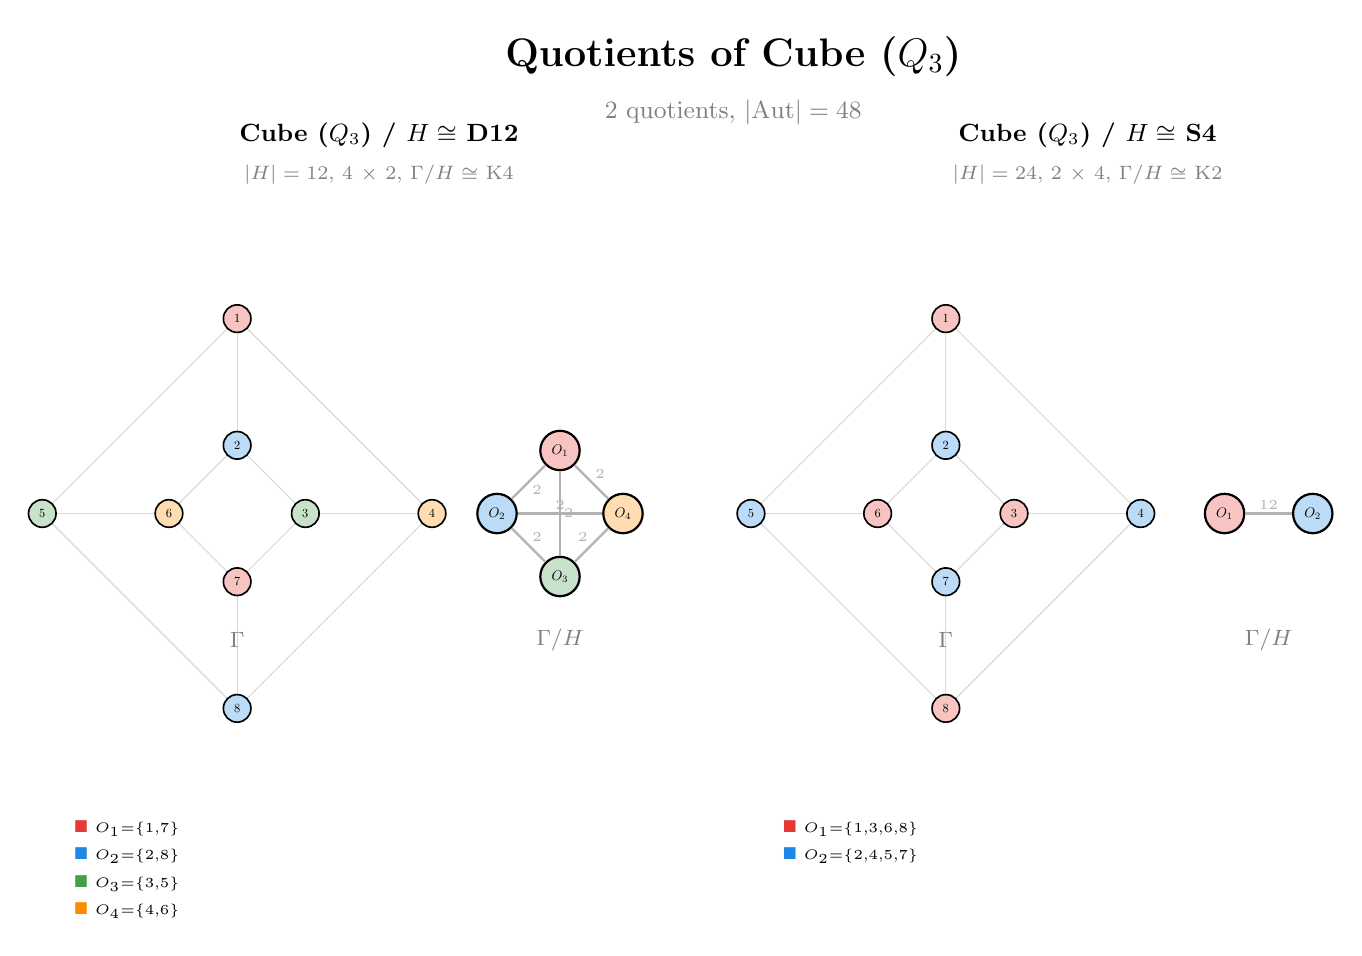
\begin{tikzpicture}[
  ov/.style={circle, draw, semithick, minimum size=3.5mm, inner sep=0pt},
  ovs/.style={circle, draw, thin, minimum size=1.8mm, inner sep=0pt},
  qv/.style={circle, draw, thick, minimum size=5mm, inner sep=0pt},
  cardtitle/.style={font=\small\bfseries},
  cardsub/.style={font=\scriptsize, text=gray},
  glabel/.style={font=\footnotesize, text=gray},
]
\node[font=\Large\bfseries] at (0, 11.5) {Quotients of Cube ($Q_3$)};
\node[font=\small, text=gray] at (0, 10.8) {2 quotients, $|\mathrm{Aut}|=48$};

% Card: Cube ($Q_3$) / H=D12
\node[cardtitle] at (-4.50,10.50) {Cube ($Q_3$) / $H \cong$ D12};
\node[cardsub] at (-4.50,10.00) {$|H|=12$, 4 $\times$ 2, $\Gamma/H \cong$ K4};
\draw[gray!30, thin] (-6.300,8.175) -- (-6.300,6.566);
\draw[gray!30, thin] (-6.300,8.175) -- (-3.825,5.700);
\draw[gray!30, thin] (-6.300,8.175) -- (-8.775,5.700);
\draw[gray!30, thin] (-6.300,6.566) -- (-5.434,5.700);
\draw[gray!30, thin] (-6.300,6.566) -- (-7.166,5.700);
\draw[gray!30, thin] (-5.434,5.700) -- (-3.825,5.700);
\draw[gray!30, thin] (-5.434,5.700) -- (-6.300,4.834);
\draw[gray!30, thin] (-3.825,5.700) -- (-6.300,3.225);
\draw[gray!30, thin] (-8.775,5.700) -- (-7.166,5.700);
\draw[gray!30, thin] (-8.775,5.700) -- (-6.300,3.225);
\draw[gray!30, thin] (-7.166,5.700) -- (-6.300,4.834);
\draw[gray!30, thin] (-6.300,4.834) -- (-6.300,3.225);
\node[ov, fill=c0!30] at (-6.300,8.175) {\scalebox{0.45}{1}};
\node[ov, fill=c1!30] at (-6.300,6.566) {\scalebox{0.45}{2}};
\node[ov, fill=c2!30] at (-5.434,5.700) {\scalebox{0.45}{3}};
\node[ov, fill=c3!30] at (-3.825,5.700) {\scalebox{0.45}{4}};
\node[ov, fill=c2!30] at (-8.775,5.700) {\scalebox{0.45}{5}};
\node[ov, fill=c3!30] at (-7.166,5.700) {\scalebox{0.45}{6}};
\node[ov, fill=c0!30] at (-6.300,4.834) {\scalebox{0.45}{7}};
\node[ov, fill=c1!30] at (-6.300,3.225) {\scalebox{0.45}{8}};
\node[glabel] at (-6.30,4.10) {$\Gamma$};
\node[qv, fill=c0!30] (c1o0) at (-2.200,6.500) {\scalebox{0.5}{$O_{1}$}};
\node[qv, fill=c1!30] (c1o1) at (-3.000,5.700) {\scalebox{0.5}{$O_{2}$}};
\node[qv, fill=c2!30] (c1o2) at (-2.200,4.900) {\scalebox{0.5}{$O_{3}$}};
\node[qv, fill=c3!30] (c1o3) at (-1.400,5.700) {\scalebox{0.5}{$O_{4}$}};
\draw[gray!60, thick] (c1o0) -- node[font=\tiny, auto, inner sep=1pt] {2} (c1o1);
\draw[gray!60, thick] (c1o0) -- node[font=\tiny, auto, inner sep=1pt] {2} (c1o2);
\draw[gray!60, thick] (c1o0) -- node[font=\tiny, auto, inner sep=1pt] {2} (c1o3);
\draw[gray!60, thick] (c1o1) -- node[font=\tiny, auto, inner sep=1pt] {2} (c1o2);
\draw[gray!60, thick] (c1o1) -- node[font=\tiny, auto, inner sep=1pt] {2} (c1o3);
\draw[gray!60, thick] (c1o2) -- node[font=\tiny, auto, inner sep=1pt] {2} (c1o3);
\node[glabel] at (-2.20,4.10) {$\Gamma/H$};
\node[anchor=west, font=\tiny] at (-8.50,1.70) {\textcolor{c0}{$\blacksquare$} $O_{1}$=\{1,7\}};
\node[anchor=west, font=\tiny] at (-8.50,1.35) {\textcolor{c1}{$\blacksquare$} $O_{2}$=\{2,8\}};
\node[anchor=west, font=\tiny] at (-8.50,1.00) {\textcolor{c2}{$\blacksquare$} $O_{3}$=\{3,5\}};
\node[anchor=west, font=\tiny] at (-8.50,0.65) {\textcolor{c3}{$\blacksquare$} $O_{4}$=\{4,6\}};

% Card: Cube ($Q_3$) / H=S4
\node[cardtitle] at (4.50,10.50) {Cube ($Q_3$) / $H \cong$ S4};
\node[cardsub] at (4.50,10.00) {$|H|=24$, 2 $\times$ 4, $\Gamma/H \cong$ K2};
\draw[gray!30, thin] (2.700,8.175) -- (2.700,6.566);
\draw[gray!30, thin] (2.700,8.175) -- (5.175,5.700);
\draw[gray!30, thin] (2.700,8.175) -- (0.225,5.700);
\draw[gray!30, thin] (2.700,6.566) -- (3.566,5.700);
\draw[gray!30, thin] (2.700,6.566) -- (1.834,5.700);
\draw[gray!30, thin] (3.566,5.700) -- (5.175,5.700);
\draw[gray!30, thin] (3.566,5.700) -- (2.700,4.834);
\draw[gray!30, thin] (5.175,5.700) -- (2.700,3.225);
\draw[gray!30, thin] (0.225,5.700) -- (1.834,5.700);
\draw[gray!30, thin] (0.225,5.700) -- (2.700,3.225);
\draw[gray!30, thin] (1.834,5.700) -- (2.700,4.834);
\draw[gray!30, thin] (2.700,4.834) -- (2.700,3.225);
\node[ov, fill=c0!30] at (2.700,8.175) {\scalebox{0.45}{1}};
\node[ov, fill=c1!30] at (2.700,6.566) {\scalebox{0.45}{2}};
\node[ov, fill=c0!30] at (3.566,5.700) {\scalebox{0.45}{3}};
\node[ov, fill=c1!30] at (5.175,5.700) {\scalebox{0.45}{4}};
\node[ov, fill=c1!30] at (0.225,5.700) {\scalebox{0.45}{5}};
\node[ov, fill=c0!30] at (1.834,5.700) {\scalebox{0.45}{6}};
\node[ov, fill=c1!30] at (2.700,4.834) {\scalebox{0.45}{7}};
\node[ov, fill=c0!30] at (2.700,3.225) {\scalebox{0.45}{8}};
\node[glabel] at (2.70,4.10) {$\Gamma$};
\node[qv, fill=c0!30] (c2o0) at (6.240,5.700) {\scalebox{0.5}{$O_{1}$}};
\node[qv, fill=c1!30] (c2o1) at (7.360,5.700) {\scalebox{0.5}{$O_{2}$}};
\draw[gray!60, thick] (c2o0) -- node[font=\tiny, auto, inner sep=1pt] {12} (c2o1);
\node[glabel] at (6.80,4.10) {$\Gamma/H$};
\node[anchor=west, font=\tiny] at (0.50,1.70) {\textcolor{c0}{$\blacksquare$} $O_{1}$=\{1,3,6,8\}};
\node[anchor=west, font=\tiny] at (0.50,1.35) {\textcolor{c1}{$\blacksquare$} $O_{2}$=\{2,4,5,7\}};
\end{tikzpicture}
\end{center}
\clearpage

\begin{center}
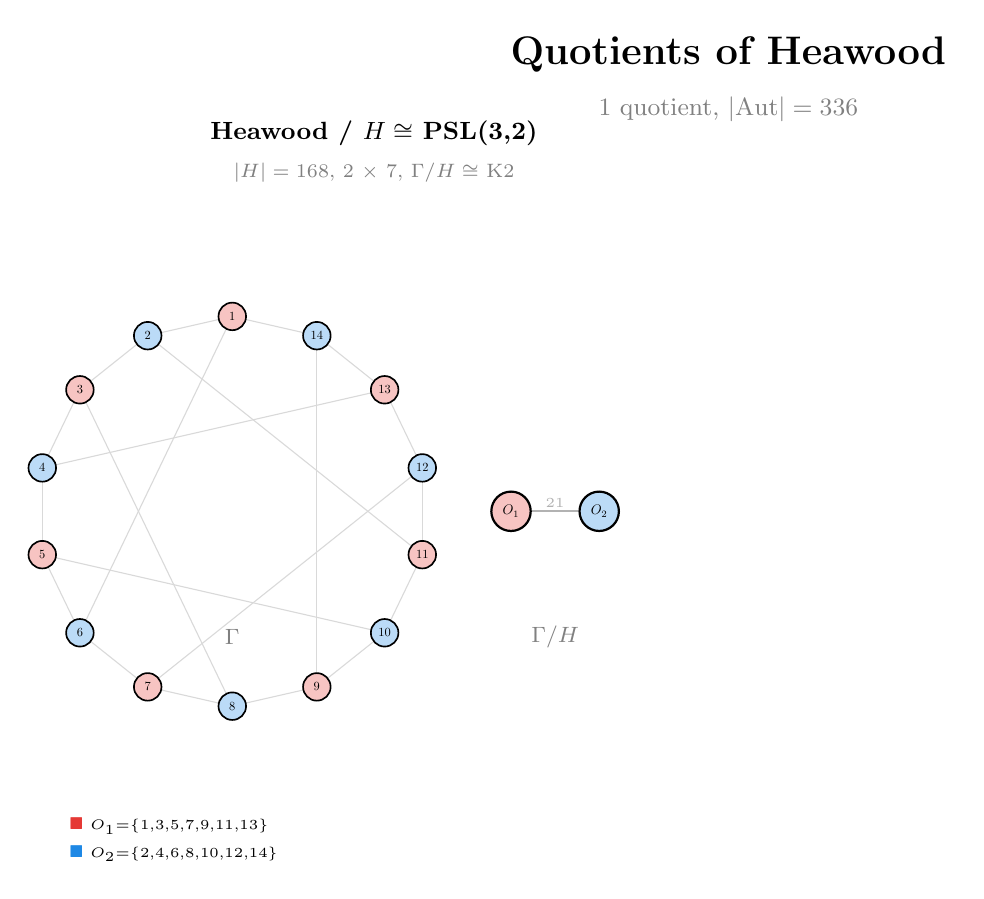
\begin{tikzpicture}[
  ov/.style={circle, draw, semithick, minimum size=3.5mm, inner sep=0pt},
  ovs/.style={circle, draw, thin, minimum size=1.8mm, inner sep=0pt},
  qv/.style={circle, draw, thick, minimum size=5mm, inner sep=0pt},
  cardtitle/.style={font=\small\bfseries},
  cardsub/.style={font=\scriptsize, text=gray},
  glabel/.style={font=\footnotesize, text=gray},
]
\node[font=\Large\bfseries] at (0, 11.5) {Quotients of Heawood};
\node[font=\small, text=gray] at (0, 10.8) {1 quotient, $|\mathrm{Aut}|=336$};

% Card: Heawood / H=PSL(3,2)
\node[cardtitle] at (-4.50,10.50) {Heawood / $H \cong$ PSL(3,2)};
\node[cardsub] at (-4.50,10.00) {$|H|=168$, 2 $\times$ 7, $\Gamma/H \cong$ K2};
\draw[gray!30, thin] (-6.300,8.175) -- (-7.374,7.930);
\draw[gray!30, thin] (-6.300,8.175) -- (-8.235,4.157);
\draw[gray!30, thin] (-6.300,8.175) -- (-5.226,7.930);
\draw[gray!30, thin] (-7.374,7.930) -- (-8.235,7.243);
\draw[gray!30, thin] (-7.374,7.930) -- (-3.887,5.149);
\draw[gray!30, thin] (-8.235,7.243) -- (-8.713,6.251);
\draw[gray!30, thin] (-8.235,7.243) -- (-6.300,3.225);
\draw[gray!30, thin] (-8.713,6.251) -- (-8.713,5.149);
\draw[gray!30, thin] (-8.713,6.251) -- (-4.365,7.243);
\draw[gray!30, thin] (-8.713,5.149) -- (-8.235,4.157);
\draw[gray!30, thin] (-8.713,5.149) -- (-4.365,4.157);
\draw[gray!30, thin] (-8.235,4.157) -- (-7.374,3.470);
\draw[gray!30, thin] (-7.374,3.470) -- (-6.300,3.225);
\draw[gray!30, thin] (-7.374,3.470) -- (-3.887,6.251);
\draw[gray!30, thin] (-6.300,3.225) -- (-5.226,3.470);
\draw[gray!30, thin] (-5.226,3.470) -- (-4.365,4.157);
\draw[gray!30, thin] (-5.226,3.470) -- (-5.226,7.930);
\draw[gray!30, thin] (-4.365,4.157) -- (-3.887,5.149);
\draw[gray!30, thin] (-3.887,5.149) -- (-3.887,6.251);
\draw[gray!30, thin] (-3.887,6.251) -- (-4.365,7.243);
\draw[gray!30, thin] (-4.365,7.243) -- (-5.226,7.930);
\node[ov, fill=c0!30] at (-6.300,8.175) {\scalebox{0.45}{1}};
\node[ov, fill=c1!30] at (-7.374,7.930) {\scalebox{0.45}{2}};
\node[ov, fill=c0!30] at (-8.235,7.243) {\scalebox{0.45}{3}};
\node[ov, fill=c1!30] at (-8.713,6.251) {\scalebox{0.45}{4}};
\node[ov, fill=c0!30] at (-8.713,5.149) {\scalebox{0.45}{5}};
\node[ov, fill=c1!30] at (-8.235,4.157) {\scalebox{0.45}{6}};
\node[ov, fill=c0!30] at (-7.374,3.470) {\scalebox{0.45}{7}};
\node[ov, fill=c1!30] at (-6.300,3.225) {\scalebox{0.45}{8}};
\node[ov, fill=c0!30] at (-5.226,3.470) {\scalebox{0.45}{9}};
\node[ov, fill=c1!30] at (-4.365,4.157) {\scalebox{0.45}{10}};
\node[ov, fill=c0!30] at (-3.887,5.149) {\scalebox{0.45}{11}};
\node[ov, fill=c1!30] at (-3.887,6.251) {\scalebox{0.45}{12}};
\node[ov, fill=c0!30] at (-4.365,7.243) {\scalebox{0.45}{13}};
\node[ov, fill=c1!30] at (-5.226,7.930) {\scalebox{0.45}{14}};
\node[glabel] at (-6.30,4.10) {$\Gamma$};
\node[qv, fill=c0!30] (c3o0) at (-2.760,5.700) {\scalebox{0.5}{$O_{1}$}};
\node[qv, fill=c1!30] (c3o1) at (-1.640,5.700) {\scalebox{0.5}{$O_{2}$}};
\draw[gray!60, thick] (c3o0) -- node[font=\tiny, auto, inner sep=1pt] {21} (c3o1);
\node[glabel] at (-2.20,4.10) {$\Gamma/H$};
\node[anchor=west, font=\tiny] at (-8.50,1.70) {\textcolor{c0}{$\blacksquare$} $O_{1}$=\{1,3,5,7,9,11,13\}};
\node[anchor=west, font=\tiny] at (-8.50,1.35) {\textcolor{c1}{$\blacksquare$} $O_{2}$=\{2,4,6,8,10,12,14\}};
\end{tikzpicture}
\end{center}
\clearpage

\begin{center}
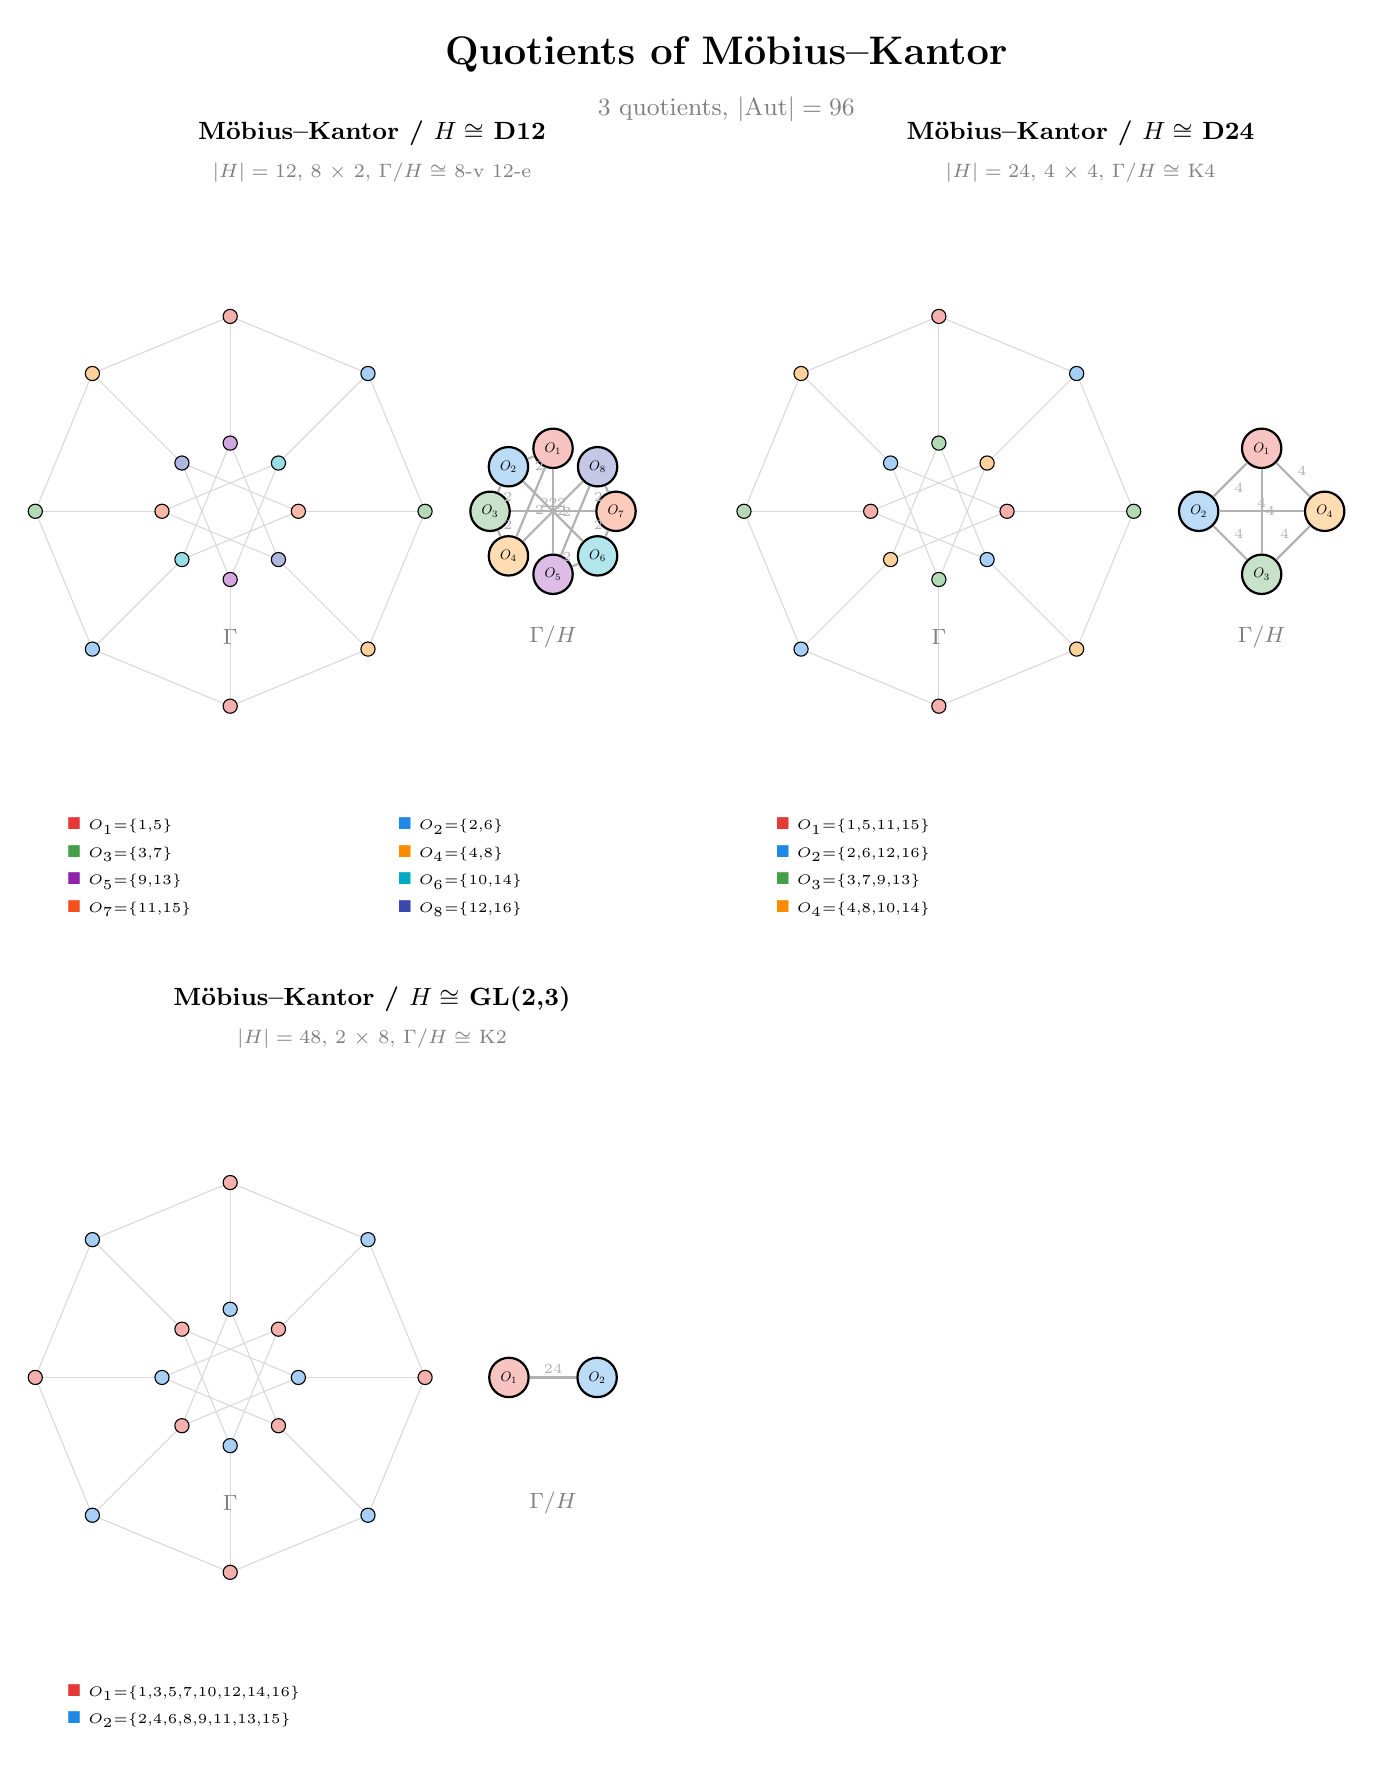
\begin{tikzpicture}[
  ov/.style={circle, draw, semithick, minimum size=3.5mm, inner sep=0pt},
  ovs/.style={circle, draw, thin, minimum size=1.8mm, inner sep=0pt},
  qv/.style={circle, draw, thick, minimum size=5mm, inner sep=0pt},
  cardtitle/.style={font=\small\bfseries},
  cardsub/.style={font=\scriptsize, text=gray},
  glabel/.style={font=\footnotesize, text=gray},
]
\node[font=\Large\bfseries] at (0, 11.5) {Quotients of M\"obius--Kantor};
\node[font=\small, text=gray] at (0, 10.8) {3 quotients, $|\mathrm{Aut}|=96$};

% Card: M\"obius--Kantor / H=D12
\node[cardtitle] at (-4.50,10.50) {M\"obius--Kantor / $H \cong$ D12};
\node[cardsub] at (-4.50,10.00) {$|H|=12$, 8 $\times$ 2, $\Gamma/H \cong$ 8-v 12-e};
\draw[gray!30, thin] (-6.300,8.175) -- (-4.550,7.450);
\draw[gray!30, thin] (-6.300,8.175) -- (-8.050,7.450);
\draw[gray!30, thin] (-6.300,8.175) -- (-6.300,6.566);
\draw[gray!30, thin] (-4.550,7.450) -- (-3.825,5.700);
\draw[gray!30, thin] (-4.550,7.450) -- (-5.687,6.313);
\draw[gray!30, thin] (-3.825,5.700) -- (-4.550,3.950);
\draw[gray!30, thin] (-3.825,5.700) -- (-5.434,5.700);
\draw[gray!30, thin] (-4.550,3.950) -- (-6.300,3.225);
\draw[gray!30, thin] (-4.550,3.950) -- (-5.687,5.087);
\draw[gray!30, thin] (-6.300,3.225) -- (-8.050,3.950);
\draw[gray!30, thin] (-6.300,3.225) -- (-6.300,4.834);
\draw[gray!30, thin] (-8.050,3.950) -- (-8.775,5.700);
\draw[gray!30, thin] (-8.050,3.950) -- (-6.913,5.087);
\draw[gray!30, thin] (-8.775,5.700) -- (-8.050,7.450);
\draw[gray!30, thin] (-8.775,5.700) -- (-7.166,5.700);
\draw[gray!30, thin] (-8.050,7.450) -- (-6.913,6.313);
\draw[gray!30, thin] (-6.300,6.566) -- (-5.687,5.087);
\draw[gray!30, thin] (-6.300,6.566) -- (-6.913,5.087);
\draw[gray!30, thin] (-5.687,6.313) -- (-6.300,4.834);
\draw[gray!30, thin] (-5.687,6.313) -- (-7.166,5.700);
\draw[gray!30, thin] (-5.434,5.700) -- (-6.913,5.087);
\draw[gray!30, thin] (-5.434,5.700) -- (-6.913,6.313);
\draw[gray!30, thin] (-5.687,5.087) -- (-7.166,5.700);
\draw[gray!30, thin] (-6.300,4.834) -- (-6.913,6.313);
\node[ovs, fill=c0!40] at (-6.300,8.175) {};
\node[ovs, fill=c1!40] at (-4.550,7.450) {};
\node[ovs, fill=c2!40] at (-3.825,5.700) {};
\node[ovs, fill=c3!40] at (-4.550,3.950) {};
\node[ovs, fill=c0!40] at (-6.300,3.225) {};
\node[ovs, fill=c1!40] at (-8.050,3.950) {};
\node[ovs, fill=c2!40] at (-8.775,5.700) {};
\node[ovs, fill=c3!40] at (-8.050,7.450) {};
\node[ovs, fill=c4!40] at (-6.300,6.566) {};
\node[ovs, fill=c5!40] at (-5.687,6.313) {};
\node[ovs, fill=c6!40] at (-5.434,5.700) {};
\node[ovs, fill=c7!40] at (-5.687,5.087) {};
\node[ovs, fill=c4!40] at (-6.300,4.834) {};
\node[ovs, fill=c5!40] at (-6.913,5.087) {};
\node[ovs, fill=c6!40] at (-7.166,5.700) {};
\node[ovs, fill=c7!40] at (-6.913,6.313) {};
\node[glabel] at (-6.30,4.10) {$\Gamma$};
\node[qv, fill=c0!30] (c4o0) at (-2.200,6.500) {\scalebox{0.5}{$O_{1}$}};
\node[qv, fill=c1!30] (c4o1) at (-2.766,6.266) {\scalebox{0.5}{$O_{2}$}};
\node[qv, fill=c2!30] (c4o2) at (-3.000,5.700) {\scalebox{0.5}{$O_{3}$}};
\node[qv, fill=c3!30] (c4o3) at (-2.766,5.134) {\scalebox{0.5}{$O_{4}$}};
\node[qv, fill=c4!30] (c4o4) at (-2.200,4.900) {\scalebox{0.5}{$O_{5}$}};
\node[qv, fill=c5!30] (c4o5) at (-1.634,5.134) {\scalebox{0.5}{$O_{6}$}};
\node[qv, fill=c6!30] (c4o6) at (-1.400,5.700) {\scalebox{0.5}{$O_{7}$}};
\node[qv, fill=c7!30] (c4o7) at (-1.634,6.266) {\scalebox{0.5}{$O_{8}$}};
\draw[gray!60, thick] (c4o0) -- node[font=\tiny, auto, inner sep=1pt] {2} (c4o1);
\draw[gray!60, thick] (c4o0) -- node[font=\tiny, auto, inner sep=1pt] {2} (c4o3);
\draw[gray!60, thick] (c4o0) -- node[font=\tiny, auto, inner sep=1pt] {2} (c4o4);
\draw[gray!60, thick] (c4o1) -- node[font=\tiny, auto, inner sep=1pt] {2} (c4o2);
\draw[gray!60, thick] (c4o1) -- node[font=\tiny, auto, inner sep=1pt] {2} (c4o5);
\draw[gray!60, thick] (c4o2) -- node[font=\tiny, auto, inner sep=1pt] {2} (c4o3);
\draw[gray!60, thick] (c4o2) -- node[font=\tiny, auto, inner sep=1pt] {2} (c4o6);
\draw[gray!60, thick] (c4o3) -- node[font=\tiny, auto, inner sep=1pt] {2} (c4o7);
\draw[gray!60, thick] (c4o4) -- node[font=\tiny, auto, inner sep=1pt] {2} (c4o5);
\draw[gray!60, thick] (c4o4) -- node[font=\tiny, auto, inner sep=1pt] {2} (c4o7);
\draw[gray!60, thick] (c4o5) -- node[font=\tiny, auto, inner sep=1pt] {2} (c4o6);
\draw[gray!60, thick] (c4o6) -- node[font=\tiny, auto, inner sep=1pt] {2} (c4o7);
\node[glabel] at (-2.20,4.10) {$\Gamma/H$};
\node[anchor=west, font=\tiny] at (-8.50,1.70) {\textcolor{c0}{$\blacksquare$} $O_{1}$=\{1,5\}};
\node[anchor=west, font=\tiny] at (-4.30,1.70) {\textcolor{c1}{$\blacksquare$} $O_{2}$=\{2,6\}};
\node[anchor=west, font=\tiny] at (-8.50,1.35) {\textcolor{c2}{$\blacksquare$} $O_{3}$=\{3,7\}};
\node[anchor=west, font=\tiny] at (-4.30,1.35) {\textcolor{c3}{$\blacksquare$} $O_{4}$=\{4,8\}};
\node[anchor=west, font=\tiny] at (-8.50,1.00) {\textcolor{c4}{$\blacksquare$} $O_{5}$=\{9,13\}};
\node[anchor=west, font=\tiny] at (-4.30,1.00) {\textcolor{c5}{$\blacksquare$} $O_{6}$=\{10,14\}};
\node[anchor=west, font=\tiny] at (-8.50,0.65) {\textcolor{c6}{$\blacksquare$} $O_{7}$=\{11,15\}};
\node[anchor=west, font=\tiny] at (-4.30,0.65) {\textcolor{c7}{$\blacksquare$} $O_{8}$=\{12,16\}};

% Card: M\"obius--Kantor / H=D24
\node[cardtitle] at (4.50,10.50) {M\"obius--Kantor / $H \cong$ D24};
\node[cardsub] at (4.50,10.00) {$|H|=24$, 4 $\times$ 4, $\Gamma/H \cong$ K4};
\draw[gray!30, thin] (2.700,8.175) -- (4.450,7.450);
\draw[gray!30, thin] (2.700,8.175) -- (0.950,7.450);
\draw[gray!30, thin] (2.700,8.175) -- (2.700,6.566);
\draw[gray!30, thin] (4.450,7.450) -- (5.175,5.700);
\draw[gray!30, thin] (4.450,7.450) -- (3.313,6.313);
\draw[gray!30, thin] (5.175,5.700) -- (4.450,3.950);
\draw[gray!30, thin] (5.175,5.700) -- (3.566,5.700);
\draw[gray!30, thin] (4.450,3.950) -- (2.700,3.225);
\draw[gray!30, thin] (4.450,3.950) -- (3.313,5.087);
\draw[gray!30, thin] (2.700,3.225) -- (0.950,3.950);
\draw[gray!30, thin] (2.700,3.225) -- (2.700,4.834);
\draw[gray!30, thin] (0.950,3.950) -- (0.225,5.700);
\draw[gray!30, thin] (0.950,3.950) -- (2.087,5.087);
\draw[gray!30, thin] (0.225,5.700) -- (0.950,7.450);
\draw[gray!30, thin] (0.225,5.700) -- (1.834,5.700);
\draw[gray!30, thin] (0.950,7.450) -- (2.087,6.313);
\draw[gray!30, thin] (2.700,6.566) -- (3.313,5.087);
\draw[gray!30, thin] (2.700,6.566) -- (2.087,5.087);
\draw[gray!30, thin] (3.313,6.313) -- (2.700,4.834);
\draw[gray!30, thin] (3.313,6.313) -- (1.834,5.700);
\draw[gray!30, thin] (3.566,5.700) -- (2.087,5.087);
\draw[gray!30, thin] (3.566,5.700) -- (2.087,6.313);
\draw[gray!30, thin] (3.313,5.087) -- (1.834,5.700);
\draw[gray!30, thin] (2.700,4.834) -- (2.087,6.313);
\node[ovs, fill=c0!40] at (2.700,8.175) {};
\node[ovs, fill=c1!40] at (4.450,7.450) {};
\node[ovs, fill=c2!40] at (5.175,5.700) {};
\node[ovs, fill=c3!40] at (4.450,3.950) {};
\node[ovs, fill=c0!40] at (2.700,3.225) {};
\node[ovs, fill=c1!40] at (0.950,3.950) {};
\node[ovs, fill=c2!40] at (0.225,5.700) {};
\node[ovs, fill=c3!40] at (0.950,7.450) {};
\node[ovs, fill=c2!40] at (2.700,6.566) {};
\node[ovs, fill=c3!40] at (3.313,6.313) {};
\node[ovs, fill=c0!40] at (3.566,5.700) {};
\node[ovs, fill=c1!40] at (3.313,5.087) {};
\node[ovs, fill=c2!40] at (2.700,4.834) {};
\node[ovs, fill=c3!40] at (2.087,5.087) {};
\node[ovs, fill=c0!40] at (1.834,5.700) {};
\node[ovs, fill=c1!40] at (2.087,6.313) {};
\node[glabel] at (2.70,4.10) {$\Gamma$};
\node[qv, fill=c0!30] (c5o0) at (6.800,6.500) {\scalebox{0.5}{$O_{1}$}};
\node[qv, fill=c1!30] (c5o1) at (6.000,5.700) {\scalebox{0.5}{$O_{2}$}};
\node[qv, fill=c2!30] (c5o2) at (6.800,4.900) {\scalebox{0.5}{$O_{3}$}};
\node[qv, fill=c3!30] (c5o3) at (7.600,5.700) {\scalebox{0.5}{$O_{4}$}};
\draw[gray!60, thick] (c5o0) -- node[font=\tiny, auto, inner sep=1pt] {4} (c5o1);
\draw[gray!60, thick] (c5o0) -- node[font=\tiny, auto, inner sep=1pt] {4} (c5o2);
\draw[gray!60, thick] (c5o0) -- node[font=\tiny, auto, inner sep=1pt] {4} (c5o3);
\draw[gray!60, thick] (c5o1) -- node[font=\tiny, auto, inner sep=1pt] {4} (c5o2);
\draw[gray!60, thick] (c5o1) -- node[font=\tiny, auto, inner sep=1pt] {4} (c5o3);
\draw[gray!60, thick] (c5o2) -- node[font=\tiny, auto, inner sep=1pt] {4} (c5o3);
\node[glabel] at (6.80,4.10) {$\Gamma/H$};
\node[anchor=west, font=\tiny] at (0.50,1.70) {\textcolor{c0}{$\blacksquare$} $O_{1}$=\{1,5,11,15\}};
\node[anchor=west, font=\tiny] at (0.50,1.35) {\textcolor{c1}{$\blacksquare$} $O_{2}$=\{2,6,12,16\}};
\node[anchor=west, font=\tiny] at (0.50,1.00) {\textcolor{c2}{$\blacksquare$} $O_{3}$=\{3,7,9,13\}};
\node[anchor=west, font=\tiny] at (0.50,0.65) {\textcolor{c3}{$\blacksquare$} $O_{4}$=\{4,8,10,14\}};

% Card: M\"obius--Kantor / H=GL(2,3)
\node[cardtitle] at (-4.50,-0.50) {M\"obius--Kantor / $H \cong$ GL(2,3)};
\node[cardsub] at (-4.50,-1.00) {$|H|=48$, 2 $\times$ 8, $\Gamma/H \cong$ K2};
\draw[gray!30, thin] (-6.300,-2.825) -- (-4.550,-3.550);
\draw[gray!30, thin] (-6.300,-2.825) -- (-8.050,-3.550);
\draw[gray!30, thin] (-6.300,-2.825) -- (-6.300,-4.434);
\draw[gray!30, thin] (-4.550,-3.550) -- (-3.825,-5.300);
\draw[gray!30, thin] (-4.550,-3.550) -- (-5.687,-4.687);
\draw[gray!30, thin] (-3.825,-5.300) -- (-4.550,-7.050);
\draw[gray!30, thin] (-3.825,-5.300) -- (-5.434,-5.300);
\draw[gray!30, thin] (-4.550,-7.050) -- (-6.300,-7.775);
\draw[gray!30, thin] (-4.550,-7.050) -- (-5.687,-5.913);
\draw[gray!30, thin] (-6.300,-7.775) -- (-8.050,-7.050);
\draw[gray!30, thin] (-6.300,-7.775) -- (-6.300,-6.166);
\draw[gray!30, thin] (-8.050,-7.050) -- (-8.775,-5.300);
\draw[gray!30, thin] (-8.050,-7.050) -- (-6.913,-5.913);
\draw[gray!30, thin] (-8.775,-5.300) -- (-8.050,-3.550);
\draw[gray!30, thin] (-8.775,-5.300) -- (-7.166,-5.300);
\draw[gray!30, thin] (-8.050,-3.550) -- (-6.913,-4.687);
\draw[gray!30, thin] (-6.300,-4.434) -- (-5.687,-5.913);
\draw[gray!30, thin] (-6.300,-4.434) -- (-6.913,-5.913);
\draw[gray!30, thin] (-5.687,-4.687) -- (-6.300,-6.166);
\draw[gray!30, thin] (-5.687,-4.687) -- (-7.166,-5.300);
\draw[gray!30, thin] (-5.434,-5.300) -- (-6.913,-5.913);
\draw[gray!30, thin] (-5.434,-5.300) -- (-6.913,-4.687);
\draw[gray!30, thin] (-5.687,-5.913) -- (-7.166,-5.300);
\draw[gray!30, thin] (-6.300,-6.166) -- (-6.913,-4.687);
\node[ovs, fill=c0!40] at (-6.300,-2.825) {};
\node[ovs, fill=c1!40] at (-4.550,-3.550) {};
\node[ovs, fill=c0!40] at (-3.825,-5.300) {};
\node[ovs, fill=c1!40] at (-4.550,-7.050) {};
\node[ovs, fill=c0!40] at (-6.300,-7.775) {};
\node[ovs, fill=c1!40] at (-8.050,-7.050) {};
\node[ovs, fill=c0!40] at (-8.775,-5.300) {};
\node[ovs, fill=c1!40] at (-8.050,-3.550) {};
\node[ovs, fill=c1!40] at (-6.300,-4.434) {};
\node[ovs, fill=c0!40] at (-5.687,-4.687) {};
\node[ovs, fill=c1!40] at (-5.434,-5.300) {};
\node[ovs, fill=c0!40] at (-5.687,-5.913) {};
\node[ovs, fill=c1!40] at (-6.300,-6.166) {};
\node[ovs, fill=c0!40] at (-6.913,-5.913) {};
\node[ovs, fill=c1!40] at (-7.166,-5.300) {};
\node[ovs, fill=c0!40] at (-6.913,-4.687) {};
\node[glabel] at (-6.30,-6.90) {$\Gamma$};
\node[qv, fill=c0!30] (c6o0) at (-2.760,-5.300) {\scalebox{0.5}{$O_{1}$}};
\node[qv, fill=c1!30] (c6o1) at (-1.640,-5.300) {\scalebox{0.5}{$O_{2}$}};
\draw[gray!60, thick] (c6o0) -- node[font=\tiny, auto, inner sep=1pt] {24} (c6o1);
\node[glabel] at (-2.20,-6.90) {$\Gamma/H$};
\node[anchor=west, font=\tiny] at (-8.50,-9.30) {\textcolor{c0}{$\blacksquare$} $O_{1}$=\{1,3,5,7,10,12,14,16\}};
\node[anchor=west, font=\tiny] at (-8.50,-9.65) {\textcolor{c1}{$\blacksquare$} $O_{2}$=\{2,4,6,8,9,11,13,15\}};
\end{tikzpicture}
\end{center}
\clearpage

\begin{center}
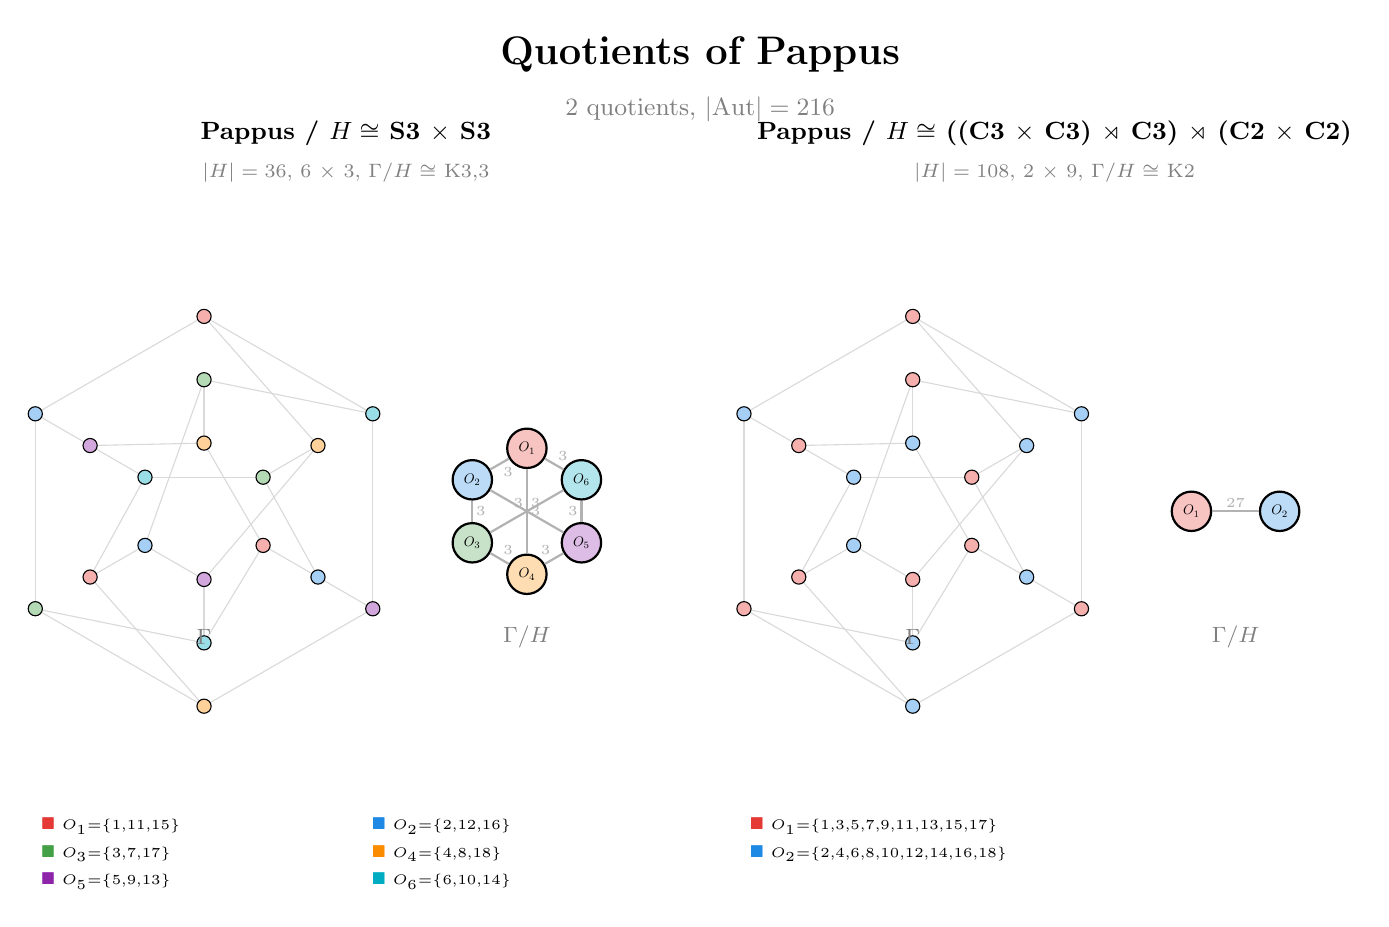
\begin{tikzpicture}[
  ov/.style={circle, draw, semithick, minimum size=3.5mm, inner sep=0pt},
  ovs/.style={circle, draw, thin, minimum size=1.8mm, inner sep=0pt},
  qv/.style={circle, draw, thick, minimum size=5mm, inner sep=0pt},
  cardtitle/.style={font=\small\bfseries},
  cardsub/.style={font=\scriptsize, text=gray},
  glabel/.style={font=\footnotesize, text=gray},
]
\node[font=\Large\bfseries] at (0, 11.5) {Quotients of Pappus};
\node[font=\small, text=gray] at (0, 10.8) {2 quotients, $|\mathrm{Aut}|=216$};

% Card: Pappus / H=S3 x S3
\node[cardtitle] at (-4.50,10.50) {Pappus / $H \cong$ S3 $\times$ S3};
\node[cardsub] at (-4.50,10.00) {$|H|=36$, 6 $\times$ 3, $\Gamma/H \cong$ K3,3};
\draw[gray!30, thin] (-6.300,8.175) -- (-8.443,6.938);
\draw[gray!30, thin] (-6.300,8.175) -- (-4.157,6.938);
\draw[gray!30, thin] (-6.300,8.175) -- (-4.853,6.535);
\draw[gray!30, thin] (-8.443,6.938) -- (-8.443,4.463);
\draw[gray!30, thin] (-8.443,6.938) -- (-7.747,6.535);
\draw[gray!30, thin] (-8.443,4.463) -- (-6.300,3.225);
\draw[gray!30, thin] (-8.443,4.463) -- (-6.300,4.029);
\draw[gray!30, thin] (-6.300,3.225) -- (-4.157,4.462);
\draw[gray!30, thin] (-6.300,3.225) -- (-7.747,4.865);
\draw[gray!30, thin] (-4.157,4.462) -- (-4.157,6.938);
\draw[gray!30, thin] (-4.157,4.462) -- (-4.853,4.865);
\draw[gray!30, thin] (-4.157,6.938) -- (-6.300,7.371);
\draw[gray!30, thin] (-6.300,7.371) -- (-6.300,6.566);
\draw[gray!30, thin] (-6.300,7.371) -- (-7.050,5.267);
\draw[gray!30, thin] (-6.300,6.566) -- (-7.747,6.535);
\draw[gray!30, thin] (-6.300,6.566) -- (-5.550,5.267);
\draw[gray!30, thin] (-7.747,6.535) -- (-7.050,6.133);
\draw[gray!30, thin] (-7.050,6.133) -- (-7.747,4.865);
\draw[gray!30, thin] (-7.050,6.133) -- (-5.550,6.133);
\draw[gray!30, thin] (-7.747,4.865) -- (-7.050,5.267);
\draw[gray!30, thin] (-7.050,5.267) -- (-6.300,4.834);
\draw[gray!30, thin] (-6.300,4.834) -- (-6.300,4.029);
\draw[gray!30, thin] (-6.300,4.834) -- (-4.853,6.535);
\draw[gray!30, thin] (-6.300,4.029) -- (-5.550,5.267);
\draw[gray!30, thin] (-5.550,5.267) -- (-4.853,4.865);
\draw[gray!30, thin] (-4.853,4.865) -- (-5.550,6.133);
\draw[gray!30, thin] (-5.550,6.133) -- (-4.853,6.535);
\node[ovs, fill=c0!40] at (-6.300,8.175) {};
\node[ovs, fill=c1!40] at (-8.443,6.938) {};
\node[ovs, fill=c2!40] at (-8.443,4.463) {};
\node[ovs, fill=c3!40] at (-6.300,3.225) {};
\node[ovs, fill=c4!40] at (-4.157,4.462) {};
\node[ovs, fill=c5!40] at (-4.157,6.938) {};
\node[ovs, fill=c2!40] at (-6.300,7.371) {};
\node[ovs, fill=c3!40] at (-6.300,6.566) {};
\node[ovs, fill=c4!40] at (-7.747,6.535) {};
\node[ovs, fill=c5!40] at (-7.050,6.133) {};
\node[ovs, fill=c0!40] at (-7.747,4.865) {};
\node[ovs, fill=c1!40] at (-7.050,5.267) {};
\node[ovs, fill=c4!40] at (-6.300,4.834) {};
\node[ovs, fill=c5!40] at (-6.300,4.029) {};
\node[ovs, fill=c0!40] at (-5.550,5.267) {};
\node[ovs, fill=c1!40] at (-4.853,4.865) {};
\node[ovs, fill=c2!40] at (-5.550,6.133) {};
\node[ovs, fill=c3!40] at (-4.853,6.535) {};
\node[glabel] at (-6.30,4.10) {$\Gamma$};
\node[qv, fill=c0!30] (c7o0) at (-2.200,6.500) {\scalebox{0.5}{$O_{1}$}};
\node[qv, fill=c1!30] (c7o1) at (-2.893,6.100) {\scalebox{0.5}{$O_{2}$}};
\node[qv, fill=c2!30] (c7o2) at (-2.893,5.300) {\scalebox{0.5}{$O_{3}$}};
\node[qv, fill=c3!30] (c7o3) at (-2.200,4.900) {\scalebox{0.5}{$O_{4}$}};
\node[qv, fill=c4!30] (c7o4) at (-1.507,5.300) {\scalebox{0.5}{$O_{5}$}};
\node[qv, fill=c5!30] (c7o5) at (-1.507,6.100) {\scalebox{0.5}{$O_{6}$}};
\draw[gray!60, thick] (c7o0) -- node[font=\tiny, auto, inner sep=1pt] {3} (c7o1);
\draw[gray!60, thick] (c7o0) -- node[font=\tiny, auto, inner sep=1pt] {3} (c7o3);
\draw[gray!60, thick] (c7o0) -- node[font=\tiny, auto, inner sep=1pt] {3} (c7o5);
\draw[gray!60, thick] (c7o1) -- node[font=\tiny, auto, inner sep=1pt] {3} (c7o2);
\draw[gray!60, thick] (c7o1) -- node[font=\tiny, auto, inner sep=1pt] {3} (c7o4);
\draw[gray!60, thick] (c7o2) -- node[font=\tiny, auto, inner sep=1pt] {3} (c7o3);
\draw[gray!60, thick] (c7o2) -- node[font=\tiny, auto, inner sep=1pt] {3} (c7o5);
\draw[gray!60, thick] (c7o3) -- node[font=\tiny, auto, inner sep=1pt] {3} (c7o4);
\draw[gray!60, thick] (c7o4) -- node[font=\tiny, auto, inner sep=1pt] {3} (c7o5);
\node[glabel] at (-2.20,4.10) {$\Gamma/H$};
\node[anchor=west, font=\tiny] at (-8.50,1.70) {\textcolor{c0}{$\blacksquare$} $O_{1}$=\{1,11,15\}};
\node[anchor=west, font=\tiny] at (-4.30,1.70) {\textcolor{c1}{$\blacksquare$} $O_{2}$=\{2,12,16\}};
\node[anchor=west, font=\tiny] at (-8.50,1.35) {\textcolor{c2}{$\blacksquare$} $O_{3}$=\{3,7,17\}};
\node[anchor=west, font=\tiny] at (-4.30,1.35) {\textcolor{c3}{$\blacksquare$} $O_{4}$=\{4,8,18\}};
\node[anchor=west, font=\tiny] at (-8.50,1.00) {\textcolor{c4}{$\blacksquare$} $O_{5}$=\{5,9,13\}};
\node[anchor=west, font=\tiny] at (-4.30,1.00) {\textcolor{c5}{$\blacksquare$} $O_{6}$=\{6,10,14\}};

% Card: Pappus / H=((C3 x C3) : C3) : (C2 x C2)
\node[cardtitle] at (4.50,10.50) {Pappus / $H \cong$ ((C3 $\times$ C3) $\rtimes$ C3) $\rtimes$ (C2 $\times$ C2)};
\node[cardsub] at (4.50,10.00) {$|H|=108$, 2 $\times$ 9, $\Gamma/H \cong$ K2};
\draw[gray!30, thin] (2.700,8.175) -- (0.557,6.938);
\draw[gray!30, thin] (2.700,8.175) -- (4.843,6.938);
\draw[gray!30, thin] (2.700,8.175) -- (4.147,6.535);
\draw[gray!30, thin] (0.557,6.938) -- (0.557,4.463);
\draw[gray!30, thin] (0.557,6.938) -- (1.253,6.535);
\draw[gray!30, thin] (0.557,4.463) -- (2.700,3.225);
\draw[gray!30, thin] (0.557,4.463) -- (2.700,4.029);
\draw[gray!30, thin] (2.700,3.225) -- (4.843,4.462);
\draw[gray!30, thin] (2.700,3.225) -- (1.253,4.865);
\draw[gray!30, thin] (4.843,4.462) -- (4.843,6.938);
\draw[gray!30, thin] (4.843,4.462) -- (4.147,4.865);
\draw[gray!30, thin] (4.843,6.938) -- (2.700,7.371);
\draw[gray!30, thin] (2.700,7.371) -- (2.700,6.566);
\draw[gray!30, thin] (2.700,7.371) -- (1.950,5.267);
\draw[gray!30, thin] (2.700,6.566) -- (1.253,6.535);
\draw[gray!30, thin] (2.700,6.566) -- (3.450,5.267);
\draw[gray!30, thin] (1.253,6.535) -- (1.950,6.133);
\draw[gray!30, thin] (1.950,6.133) -- (1.253,4.865);
\draw[gray!30, thin] (1.950,6.133) -- (3.450,6.133);
\draw[gray!30, thin] (1.253,4.865) -- (1.950,5.267);
\draw[gray!30, thin] (1.950,5.267) -- (2.700,4.834);
\draw[gray!30, thin] (2.700,4.834) -- (2.700,4.029);
\draw[gray!30, thin] (2.700,4.834) -- (4.147,6.535);
\draw[gray!30, thin] (2.700,4.029) -- (3.450,5.267);
\draw[gray!30, thin] (3.450,5.267) -- (4.147,4.865);
\draw[gray!30, thin] (4.147,4.865) -- (3.450,6.133);
\draw[gray!30, thin] (3.450,6.133) -- (4.147,6.535);
\node[ovs, fill=c0!40] at (2.700,8.175) {};
\node[ovs, fill=c1!40] at (0.557,6.938) {};
\node[ovs, fill=c0!40] at (0.557,4.463) {};
\node[ovs, fill=c1!40] at (2.700,3.225) {};
\node[ovs, fill=c0!40] at (4.843,4.462) {};
\node[ovs, fill=c1!40] at (4.843,6.938) {};
\node[ovs, fill=c0!40] at (2.700,7.371) {};
\node[ovs, fill=c1!40] at (2.700,6.566) {};
\node[ovs, fill=c0!40] at (1.253,6.535) {};
\node[ovs, fill=c1!40] at (1.950,6.133) {};
\node[ovs, fill=c0!40] at (1.253,4.865) {};
\node[ovs, fill=c1!40] at (1.950,5.267) {};
\node[ovs, fill=c0!40] at (2.700,4.834) {};
\node[ovs, fill=c1!40] at (2.700,4.029) {};
\node[ovs, fill=c0!40] at (3.450,5.267) {};
\node[ovs, fill=c1!40] at (4.147,4.865) {};
\node[ovs, fill=c0!40] at (3.450,6.133) {};
\node[ovs, fill=c1!40] at (4.147,6.535) {};
\node[glabel] at (2.70,4.10) {$\Gamma$};
\node[qv, fill=c0!30] (c8o0) at (6.240,5.700) {\scalebox{0.5}{$O_{1}$}};
\node[qv, fill=c1!30] (c8o1) at (7.360,5.700) {\scalebox{0.5}{$O_{2}$}};
\draw[gray!60, thick] (c8o0) -- node[font=\tiny, auto, inner sep=1pt] {27} (c8o1);
\node[glabel] at (6.80,4.10) {$\Gamma/H$};
\node[anchor=west, font=\tiny] at (0.50,1.70) {\textcolor{c0}{$\blacksquare$} $O_{1}$=\{1,3,5,7,9,11,13,15,17\}};
\node[anchor=west, font=\tiny] at (0.50,1.35) {\textcolor{c1}{$\blacksquare$} $O_{2}$=\{2,4,6,8,10,12,14,16,18\}};
\end{tikzpicture}
\end{center}
\clearpage

\begin{center}
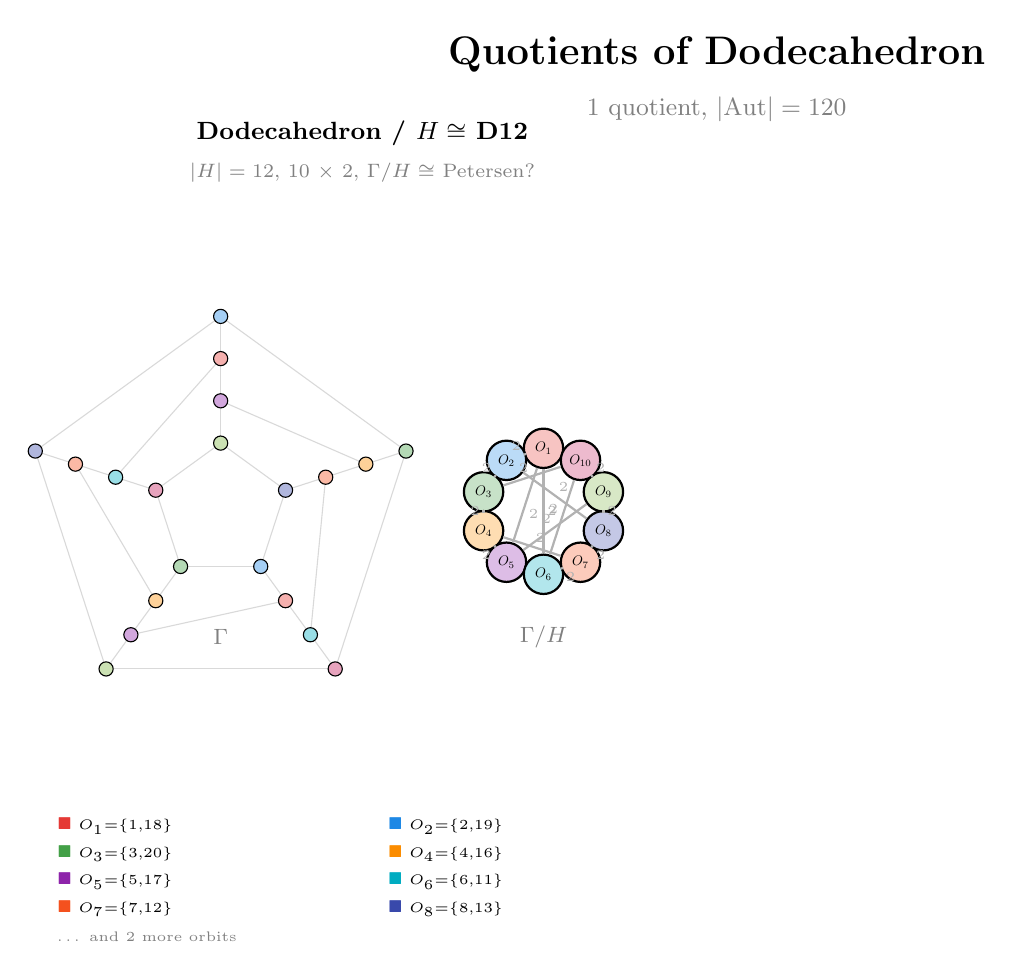
\begin{tikzpicture}[
  ov/.style={circle, draw, semithick, minimum size=3.5mm, inner sep=0pt},
  ovs/.style={circle, draw, thin, minimum size=1.8mm, inner sep=0pt},
  qv/.style={circle, draw, thick, minimum size=5mm, inner sep=0pt},
  cardtitle/.style={font=\small\bfseries},
  cardsub/.style={font=\scriptsize, text=gray},
  glabel/.style={font=\footnotesize, text=gray},
]
\node[font=\Large\bfseries] at (0, 11.5) {Quotients of Dodecahedron};
\node[font=\small, text=gray] at (0, 10.8) {1 quotient, $|\mathrm{Aut}|=120$};

% Card: Dodecahedron / H=D12
\node[cardtitle] at (-4.50,10.50) {Dodecahedron / $H \cong$ D12};
\node[cardsub] at (-4.50,10.00) {$|H|=12$, 10 $\times$ 2, $\Gamma/H \cong$ Petersen?};
\draw[gray!30, thin] (-6.300,7.639) -- (-6.300,8.175);
\draw[gray!30, thin] (-6.300,7.639) -- (-6.300,7.103);
\draw[gray!30, thin] (-6.300,7.639) -- (-7.634,6.133);
\draw[gray!30, thin] (-6.300,8.175) -- (-3.946,6.465);
\draw[gray!30, thin] (-6.300,8.175) -- (-8.654,6.465);
\draw[gray!30, thin] (-3.946,6.465) -- (-4.456,6.299);
\draw[gray!30, thin] (-3.946,6.465) -- (-4.845,3.698);
\draw[gray!30, thin] (-4.456,6.299) -- (-6.300,7.103);
\draw[gray!30, thin] (-4.456,6.299) -- (-4.966,6.133);
\draw[gray!30, thin] (-6.300,7.103) -- (-6.300,6.566);
\draw[gray!30, thin] (-7.634,6.133) -- (-8.144,6.299);
\draw[gray!30, thin] (-7.634,6.133) -- (-7.124,5.968);
\draw[gray!30, thin] (-8.144,6.299) -- (-8.654,6.465);
\draw[gray!30, thin] (-8.144,6.299) -- (-7.124,4.565);
\draw[gray!30, thin] (-8.654,6.465) -- (-7.755,3.698);
\draw[gray!30, thin] (-7.755,3.698) -- (-4.845,3.698);
\draw[gray!30, thin] (-7.755,3.698) -- (-7.440,4.132);
\draw[gray!30, thin] (-4.845,3.698) -- (-5.160,4.132);
\draw[gray!30, thin] (-5.160,4.132) -- (-4.966,6.133);
\draw[gray!30, thin] (-5.160,4.132) -- (-5.476,4.565);
\draw[gray!30, thin] (-4.966,6.133) -- (-5.476,5.968);
\draw[gray!30, thin] (-5.476,5.968) -- (-6.300,6.566);
\draw[gray!30, thin] (-5.476,5.968) -- (-5.791,4.999);
\draw[gray!30, thin] (-6.300,6.566) -- (-7.124,5.968);
\draw[gray!30, thin] (-7.124,5.968) -- (-6.809,4.999);
\draw[gray!30, thin] (-7.124,4.565) -- (-7.440,4.132);
\draw[gray!30, thin] (-7.124,4.565) -- (-6.809,4.999);
\draw[gray!30, thin] (-7.440,4.132) -- (-5.476,4.565);
\draw[gray!30, thin] (-5.476,4.565) -- (-5.791,4.999);
\draw[gray!30, thin] (-5.791,4.999) -- (-6.809,4.999);
\node[ovs, fill=c0!40] at (-6.300,7.639) {};
\node[ovs, fill=c1!40] at (-6.300,8.175) {};
\node[ovs, fill=c2!40] at (-3.946,6.465) {};
\node[ovs, fill=c3!40] at (-4.456,6.299) {};
\node[ovs, fill=c4!40] at (-6.300,7.103) {};
\node[ovs, fill=c5!40] at (-7.634,6.133) {};
\node[ovs, fill=c6!40] at (-8.144,6.299) {};
\node[ovs, fill=c7!40] at (-8.654,6.465) {};
\node[ovs, fill=c8!40] at (-7.755,3.698) {};
\node[ovs, fill=c9!40] at (-4.845,3.698) {};
\node[ovs, fill=c5!40] at (-5.160,4.132) {};
\node[ovs, fill=c6!40] at (-4.966,6.133) {};
\node[ovs, fill=c7!40] at (-5.476,5.968) {};
\node[ovs, fill=c8!40] at (-6.300,6.566) {};
\node[ovs, fill=c9!40] at (-7.124,5.968) {};
\node[ovs, fill=c3!40] at (-7.124,4.565) {};
\node[ovs, fill=c4!40] at (-7.440,4.132) {};
\node[ovs, fill=c0!40] at (-5.476,4.565) {};
\node[ovs, fill=c1!40] at (-5.791,4.999) {};
\node[ovs, fill=c2!40] at (-6.809,4.999) {};
\node[glabel] at (-6.30,4.10) {$\Gamma$};
\node[qv, fill=c0!30] (c9o0) at (-2.200,6.500) {\scalebox{0.5}{$O_{1}$}};
\node[qv, fill=c1!30] (c9o1) at (-2.670,6.347) {\scalebox{0.5}{$O_{2}$}};
\node[qv, fill=c2!30] (c9o2) at (-2.961,5.947) {\scalebox{0.5}{$O_{3}$}};
\node[qv, fill=c3!30] (c9o3) at (-2.961,5.453) {\scalebox{0.5}{$O_{4}$}};
\node[qv, fill=c4!30] (c9o4) at (-2.670,5.053) {\scalebox{0.5}{$O_{5}$}};
\node[qv, fill=c5!30] (c9o5) at (-2.200,4.900) {\scalebox{0.5}{$O_{6}$}};
\node[qv, fill=c6!30] (c9o6) at (-1.730,5.053) {\scalebox{0.5}{$O_{7}$}};
\node[qv, fill=c7!30] (c9o7) at (-1.439,5.453) {\scalebox{0.5}{$O_{8}$}};
\node[qv, fill=c8!30] (c9o8) at (-1.439,5.947) {\scalebox{0.5}{$O_{9}$}};
\node[qv, fill=c9!30] (c9o9) at (-1.730,6.347) {\scalebox{0.5}{$O_{10}$}};
\draw[gray!60, thick] (c9o0) -- node[font=\tiny, auto, inner sep=1pt] {2} (c9o1);
\draw[gray!60, thick] (c9o0) -- node[font=\tiny, auto, inner sep=1pt] {2} (c9o4);
\draw[gray!60, thick] (c9o0) -- node[font=\tiny, auto, inner sep=1pt] {2} (c9o5);
\draw[gray!60, thick] (c9o1) -- node[font=\tiny, auto, inner sep=1pt] {2} (c9o2);
\draw[gray!60, thick] (c9o1) -- node[font=\tiny, auto, inner sep=1pt] {2} (c9o7);
\draw[gray!60, thick] (c9o2) -- node[font=\tiny, auto, inner sep=1pt] {2} (c9o3);
\draw[gray!60, thick] (c9o2) -- node[font=\tiny, auto, inner sep=1pt] {2} (c9o9);
\draw[gray!60, thick] (c9o3) -- node[font=\tiny, auto, inner sep=1pt] {2} (c9o4);
\draw[gray!60, thick] (c9o3) -- node[font=\tiny, auto, inner sep=1pt] {2} (c9o6);
\draw[gray!60, thick] (c9o4) -- node[font=\tiny, auto, inner sep=1pt] {2} (c9o8);
\draw[gray!60, thick] (c9o5) -- node[font=\tiny, auto, inner sep=1pt] {2} (c9o6);
\draw[gray!60, thick] (c9o5) -- node[font=\tiny, auto, inner sep=1pt] {2} (c9o9);
\draw[gray!60, thick] (c9o6) -- node[font=\tiny, auto, inner sep=1pt] {2} (c9o7);
\draw[gray!60, thick] (c9o7) -- node[font=\tiny, auto, inner sep=1pt] {2} (c9o8);
\draw[gray!60, thick] (c9o8) -- node[font=\tiny, auto, inner sep=1pt] {2} (c9o9);
\node[glabel] at (-2.20,4.10) {$\Gamma/H$};
\node[anchor=west, font=\tiny] at (-8.50,1.70) {\textcolor{c0}{$\blacksquare$} $O_{1}$=\{1,18\}};
\node[anchor=west, font=\tiny] at (-4.30,1.70) {\textcolor{c1}{$\blacksquare$} $O_{2}$=\{2,19\}};
\node[anchor=west, font=\tiny] at (-8.50,1.35) {\textcolor{c2}{$\blacksquare$} $O_{3}$=\{3,20\}};
\node[anchor=west, font=\tiny] at (-4.30,1.35) {\textcolor{c3}{$\blacksquare$} $O_{4}$=\{4,16\}};
\node[anchor=west, font=\tiny] at (-8.50,1.00) {\textcolor{c4}{$\blacksquare$} $O_{5}$=\{5,17\}};
\node[anchor=west, font=\tiny] at (-4.30,1.00) {\textcolor{c5}{$\blacksquare$} $O_{6}$=\{6,11\}};
\node[anchor=west, font=\tiny] at (-8.50,0.65) {\textcolor{c6}{$\blacksquare$} $O_{7}$=\{7,12\}};
\node[anchor=west, font=\tiny] at (-4.30,0.65) {\textcolor{c7}{$\blacksquare$} $O_{8}$=\{8,13\}};
\node[anchor=west, font=\tiny, text=gray] at (-8.50,0.30) {\ldots\ and 2 more orbits};
\end{tikzpicture}
\end{center}
\clearpage

\begin{center}
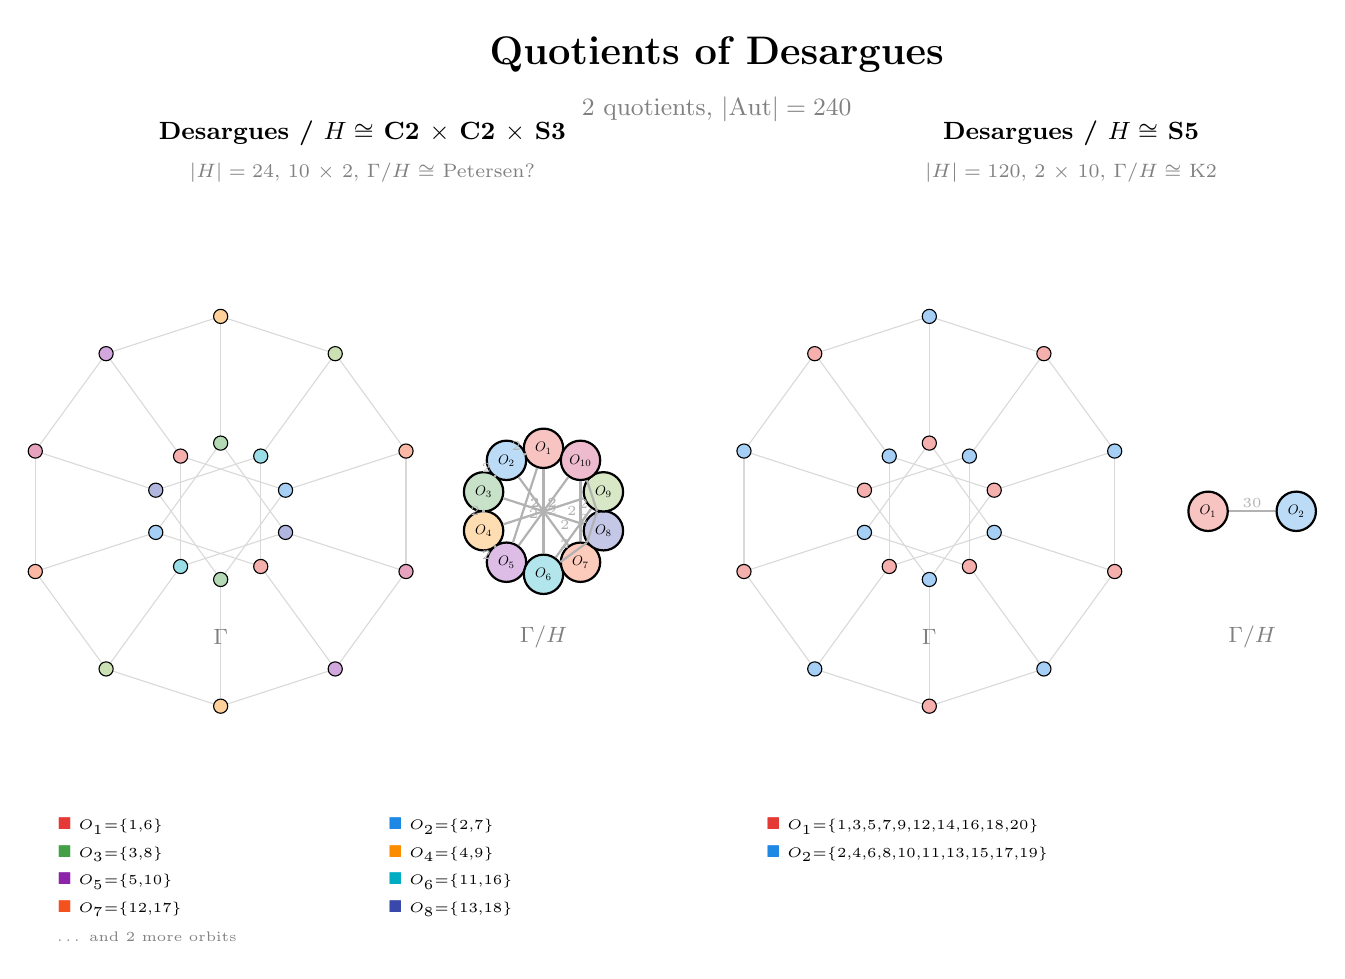
\begin{tikzpicture}[
  ov/.style={circle, draw, semithick, minimum size=3.5mm, inner sep=0pt},
  ovs/.style={circle, draw, thin, minimum size=1.8mm, inner sep=0pt},
  qv/.style={circle, draw, thick, minimum size=5mm, inner sep=0pt},
  cardtitle/.style={font=\small\bfseries},
  cardsub/.style={font=\scriptsize, text=gray},
  glabel/.style={font=\footnotesize, text=gray},
]
\node[font=\Large\bfseries] at (0, 11.5) {Quotients of Desargues};
\node[font=\small, text=gray] at (0, 10.8) {2 quotients, $|\mathrm{Aut}|=240$};

% Card: Desargues / H=C2 x C2 x S3
\node[cardtitle] at (-4.50,10.50) {Desargues / $H \cong$ C2 $\times$ C2 $\times$ S3};
\node[cardsub] at (-4.50,10.00) {$|H|=24$, 10 $\times$ 2, $\Gamma/H \cong$ Petersen?};
\draw[gray!30, thin] (-5.791,4.999) -- (-7.124,5.432);
\draw[gray!30, thin] (-5.791,4.999) -- (-4.845,3.698);
\draw[gray!30, thin] (-5.791,4.999) -- (-5.791,6.401);
\draw[gray!30, thin] (-7.124,5.432) -- (-6.300,6.566);
\draw[gray!30, thin] (-7.124,5.432) -- (-8.654,4.935);
\draw[gray!30, thin] (-6.300,6.566) -- (-6.300,8.175);
\draw[gray!30, thin] (-6.300,6.566) -- (-5.476,5.432);
\draw[gray!30, thin] (-6.300,8.175) -- (-7.755,7.702);
\draw[gray!30, thin] (-6.300,8.175) -- (-4.845,7.702);
\draw[gray!30, thin] (-7.755,7.702) -- (-6.809,6.401);
\draw[gray!30, thin] (-7.755,7.702) -- (-8.654,6.465);
\draw[gray!30, thin] (-6.809,6.401) -- (-5.476,5.968);
\draw[gray!30, thin] (-6.809,6.401) -- (-6.809,4.999);
\draw[gray!30, thin] (-5.476,5.968) -- (-6.300,4.834);
\draw[gray!30, thin] (-5.476,5.968) -- (-3.946,6.465);
\draw[gray!30, thin] (-6.300,4.834) -- (-6.300,3.225);
\draw[gray!30, thin] (-6.300,4.834) -- (-7.124,5.968);
\draw[gray!30, thin] (-6.300,3.225) -- (-4.845,3.698);
\draw[gray!30, thin] (-6.300,3.225) -- (-7.755,3.698);
\draw[gray!30, thin] (-4.845,3.698) -- (-3.946,4.935);
\draw[gray!30, thin] (-5.791,6.401) -- (-4.845,7.702);
\draw[gray!30, thin] (-5.791,6.401) -- (-7.124,5.968);
\draw[gray!30, thin] (-8.654,4.935) -- (-8.654,6.465);
\draw[gray!30, thin] (-8.654,4.935) -- (-7.755,3.698);
\draw[gray!30, thin] (-5.476,5.432) -- (-6.809,4.999);
\draw[gray!30, thin] (-5.476,5.432) -- (-3.946,4.935);
\draw[gray!30, thin] (-4.845,7.702) -- (-3.946,6.465);
\draw[gray!30, thin] (-8.654,6.465) -- (-7.124,5.968);
\draw[gray!30, thin] (-6.809,4.999) -- (-7.755,3.698);
\draw[gray!30, thin] (-3.946,6.465) -- (-3.946,4.935);
\node[ovs, fill=c0!40] at (-5.791,4.999) {};
\node[ovs, fill=c1!40] at (-7.124,5.432) {};
\node[ovs, fill=c2!40] at (-6.300,6.566) {};
\node[ovs, fill=c3!40] at (-6.300,8.175) {};
\node[ovs, fill=c4!40] at (-7.755,7.702) {};
\node[ovs, fill=c0!40] at (-6.809,6.401) {};
\node[ovs, fill=c1!40] at (-5.476,5.968) {};
\node[ovs, fill=c2!40] at (-6.300,4.834) {};
\node[ovs, fill=c3!40] at (-6.300,3.225) {};
\node[ovs, fill=c4!40] at (-4.845,3.698) {};
\node[ovs, fill=c5!40] at (-5.791,6.401) {};
\node[ovs, fill=c6!40] at (-8.654,4.935) {};
\node[ovs, fill=c7!40] at (-5.476,5.432) {};
\node[ovs, fill=c8!40] at (-4.845,7.702) {};
\node[ovs, fill=c9!40] at (-8.654,6.465) {};
\node[ovs, fill=c5!40] at (-6.809,4.999) {};
\node[ovs, fill=c6!40] at (-3.946,6.465) {};
\node[ovs, fill=c7!40] at (-7.124,5.968) {};
\node[ovs, fill=c8!40] at (-7.755,3.698) {};
\node[ovs, fill=c9!40] at (-3.946,4.935) {};
\node[glabel] at (-6.30,4.10) {$\Gamma$};
\node[qv, fill=c0!30] (c10o0) at (-2.200,6.500) {\scalebox{0.5}{$O_{1}$}};
\node[qv, fill=c1!30] (c10o1) at (-2.670,6.347) {\scalebox{0.5}{$O_{2}$}};
\node[qv, fill=c2!30] (c10o2) at (-2.961,5.947) {\scalebox{0.5}{$O_{3}$}};
\node[qv, fill=c3!30] (c10o3) at (-2.961,5.453) {\scalebox{0.5}{$O_{4}$}};
\node[qv, fill=c4!30] (c10o4) at (-2.670,5.053) {\scalebox{0.5}{$O_{5}$}};
\node[qv, fill=c5!30] (c10o5) at (-2.200,4.900) {\scalebox{0.5}{$O_{6}$}};
\node[qv, fill=c6!30] (c10o6) at (-1.730,5.053) {\scalebox{0.5}{$O_{7}$}};
\node[qv, fill=c7!30] (c10o7) at (-1.439,5.453) {\scalebox{0.5}{$O_{8}$}};
\node[qv, fill=c8!30] (c10o8) at (-1.439,5.947) {\scalebox{0.5}{$O_{9}$}};
\node[qv, fill=c9!30] (c10o9) at (-1.730,6.347) {\scalebox{0.5}{$O_{10}$}};
\draw[gray!60, thick] (c10o0) -- node[font=\tiny, auto, inner sep=1pt] {2} (c10o1);
\draw[gray!60, thick] (c10o0) -- node[font=\tiny, auto, inner sep=1pt] {2} (c10o4);
\draw[gray!60, thick] (c10o0) -- node[font=\tiny, auto, inner sep=1pt] {2} (c10o5);
\draw[gray!60, thick] (c10o1) -- node[font=\tiny, auto, inner sep=1pt] {2} (c10o2);
\draw[gray!60, thick] (c10o1) -- node[font=\tiny, auto, inner sep=1pt] {2} (c10o6);
\draw[gray!60, thick] (c10o2) -- node[font=\tiny, auto, inner sep=1pt] {2} (c10o3);
\draw[gray!60, thick] (c10o2) -- node[font=\tiny, auto, inner sep=1pt] {2} (c10o7);
\draw[gray!60, thick] (c10o3) -- node[font=\tiny, auto, inner sep=1pt] {2} (c10o4);
\draw[gray!60, thick] (c10o3) -- node[font=\tiny, auto, inner sep=1pt] {2} (c10o8);
\draw[gray!60, thick] (c10o4) -- node[font=\tiny, auto, inner sep=1pt] {2} (c10o9);
\draw[gray!60, thick] (c10o5) -- node[font=\tiny, auto, inner sep=1pt] {2} (c10o7);
\draw[gray!60, thick] (c10o5) -- node[font=\tiny, auto, inner sep=1pt] {2} (c10o8);
\draw[gray!60, thick] (c10o6) -- node[font=\tiny, auto, inner sep=1pt] {2} (c10o8);
\draw[gray!60, thick] (c10o6) -- node[font=\tiny, auto, inner sep=1pt] {2} (c10o9);
\draw[gray!60, thick] (c10o7) -- node[font=\tiny, auto, inner sep=1pt] {2} (c10o9);
\node[glabel] at (-2.20,4.10) {$\Gamma/H$};
\node[anchor=west, font=\tiny] at (-8.50,1.70) {\textcolor{c0}{$\blacksquare$} $O_{1}$=\{1,6\}};
\node[anchor=west, font=\tiny] at (-4.30,1.70) {\textcolor{c1}{$\blacksquare$} $O_{2}$=\{2,7\}};
\node[anchor=west, font=\tiny] at (-8.50,1.35) {\textcolor{c2}{$\blacksquare$} $O_{3}$=\{3,8\}};
\node[anchor=west, font=\tiny] at (-4.30,1.35) {\textcolor{c3}{$\blacksquare$} $O_{4}$=\{4,9\}};
\node[anchor=west, font=\tiny] at (-8.50,1.00) {\textcolor{c4}{$\blacksquare$} $O_{5}$=\{5,10\}};
\node[anchor=west, font=\tiny] at (-4.30,1.00) {\textcolor{c5}{$\blacksquare$} $O_{6}$=\{11,16\}};
\node[anchor=west, font=\tiny] at (-8.50,0.65) {\textcolor{c6}{$\blacksquare$} $O_{7}$=\{12,17\}};
\node[anchor=west, font=\tiny] at (-4.30,0.65) {\textcolor{c7}{$\blacksquare$} $O_{8}$=\{13,18\}};
\node[anchor=west, font=\tiny, text=gray] at (-8.50,0.30) {\ldots\ and 2 more orbits};

% Card: Desargues / H=S5
\node[cardtitle] at (4.50,10.50) {Desargues / $H \cong$ S5};
\node[cardsub] at (4.50,10.00) {$|H|=120$, 2 $\times$ 10, $\Gamma/H \cong$ K2};
\draw[gray!30, thin] (3.209,4.999) -- (1.876,5.432);
\draw[gray!30, thin] (3.209,4.999) -- (4.155,3.698);
\draw[gray!30, thin] (3.209,4.999) -- (3.209,6.401);
\draw[gray!30, thin] (1.876,5.432) -- (2.700,6.566);
\draw[gray!30, thin] (1.876,5.432) -- (0.346,4.935);
\draw[gray!30, thin] (2.700,6.566) -- (2.700,8.175);
\draw[gray!30, thin] (2.700,6.566) -- (3.524,5.432);
\draw[gray!30, thin] (2.700,8.175) -- (1.245,7.702);
\draw[gray!30, thin] (2.700,8.175) -- (4.155,7.702);
\draw[gray!30, thin] (1.245,7.702) -- (2.191,6.401);
\draw[gray!30, thin] (1.245,7.702) -- (0.346,6.465);
\draw[gray!30, thin] (2.191,6.401) -- (3.524,5.968);
\draw[gray!30, thin] (2.191,6.401) -- (2.191,4.999);
\draw[gray!30, thin] (3.524,5.968) -- (2.700,4.834);
\draw[gray!30, thin] (3.524,5.968) -- (5.054,6.465);
\draw[gray!30, thin] (2.700,4.834) -- (2.700,3.225);
\draw[gray!30, thin] (2.700,4.834) -- (1.876,5.968);
\draw[gray!30, thin] (2.700,3.225) -- (4.155,3.698);
\draw[gray!30, thin] (2.700,3.225) -- (1.245,3.698);
\draw[gray!30, thin] (4.155,3.698) -- (5.054,4.935);
\draw[gray!30, thin] (3.209,6.401) -- (4.155,7.702);
\draw[gray!30, thin] (3.209,6.401) -- (1.876,5.968);
\draw[gray!30, thin] (0.346,4.935) -- (0.346,6.465);
\draw[gray!30, thin] (0.346,4.935) -- (1.245,3.698);
\draw[gray!30, thin] (3.524,5.432) -- (2.191,4.999);
\draw[gray!30, thin] (3.524,5.432) -- (5.054,4.935);
\draw[gray!30, thin] (4.155,7.702) -- (5.054,6.465);
\draw[gray!30, thin] (0.346,6.465) -- (1.876,5.968);
\draw[gray!30, thin] (2.191,4.999) -- (1.245,3.698);
\draw[gray!30, thin] (5.054,6.465) -- (5.054,4.935);
\node[ovs, fill=c0!40] at (3.209,4.999) {};
\node[ovs, fill=c1!40] at (1.876,5.432) {};
\node[ovs, fill=c0!40] at (2.700,6.566) {};
\node[ovs, fill=c1!40] at (2.700,8.175) {};
\node[ovs, fill=c0!40] at (1.245,7.702) {};
\node[ovs, fill=c1!40] at (2.191,6.401) {};
\node[ovs, fill=c0!40] at (3.524,5.968) {};
\node[ovs, fill=c1!40] at (2.700,4.834) {};
\node[ovs, fill=c0!40] at (2.700,3.225) {};
\node[ovs, fill=c1!40] at (4.155,3.698) {};
\node[ovs, fill=c1!40] at (3.209,6.401) {};
\node[ovs, fill=c0!40] at (0.346,4.935) {};
\node[ovs, fill=c1!40] at (3.524,5.432) {};
\node[ovs, fill=c0!40] at (4.155,7.702) {};
\node[ovs, fill=c1!40] at (0.346,6.465) {};
\node[ovs, fill=c0!40] at (2.191,4.999) {};
\node[ovs, fill=c1!40] at (5.054,6.465) {};
\node[ovs, fill=c0!40] at (1.876,5.968) {};
\node[ovs, fill=c1!40] at (1.245,3.698) {};
\node[ovs, fill=c0!40] at (5.054,4.935) {};
\node[glabel] at (2.70,4.10) {$\Gamma$};
\node[qv, fill=c0!30] (c11o0) at (6.240,5.700) {\scalebox{0.5}{$O_{1}$}};
\node[qv, fill=c1!30] (c11o1) at (7.360,5.700) {\scalebox{0.5}{$O_{2}$}};
\draw[gray!60, thick] (c11o0) -- node[font=\tiny, auto, inner sep=1pt] {30} (c11o1);
\node[glabel] at (6.80,4.10) {$\Gamma/H$};
\node[anchor=west, font=\tiny] at (0.50,1.70) {\textcolor{c0}{$\blacksquare$} $O_{1}$=\{1,3,5,7,9,12,14,16,18,20\}};
\node[anchor=west, font=\tiny] at (0.50,1.35) {\textcolor{c1}{$\blacksquare$} $O_{2}$=\{2,4,6,8,10,11,13,15,17,19\}};
\end{tikzpicture}
\end{center}
\clearpage

\begin{center}
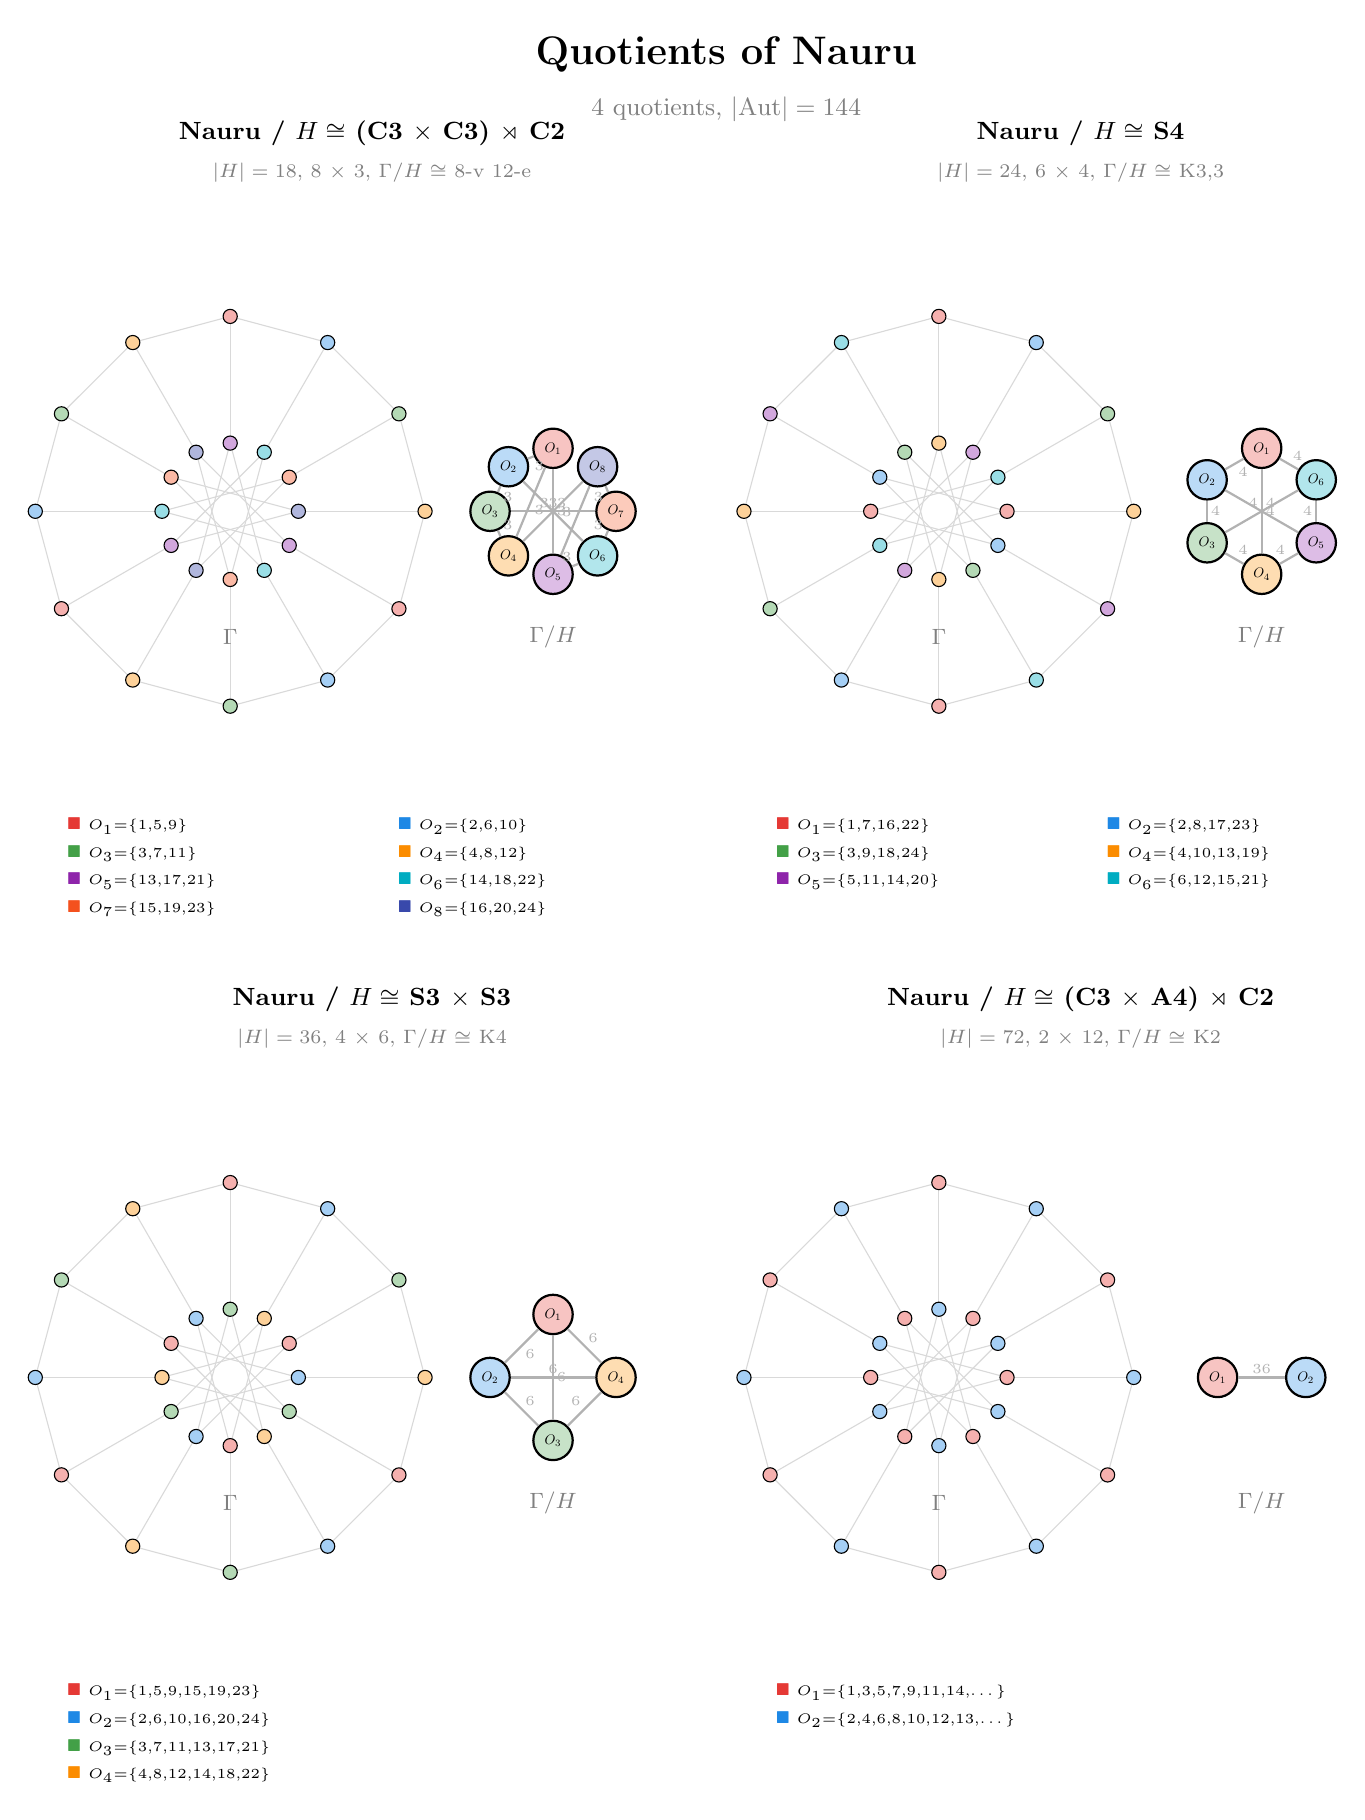
\begin{tikzpicture}[
  ov/.style={circle, draw, semithick, minimum size=3.5mm, inner sep=0pt},
  ovs/.style={circle, draw, thin, minimum size=1.8mm, inner sep=0pt},
  qv/.style={circle, draw, thick, minimum size=5mm, inner sep=0pt},
  cardtitle/.style={font=\small\bfseries},
  cardsub/.style={font=\scriptsize, text=gray},
  glabel/.style={font=\footnotesize, text=gray},
]
\node[font=\Large\bfseries] at (0, 11.5) {Quotients of Nauru};
\node[font=\small, text=gray] at (0, 10.8) {4 quotients, $|\mathrm{Aut}|=144$};

% Card: Nauru / H=(C3 x C3) : C2
\node[cardtitle] at (-4.50,10.50) {Nauru / $H \cong$ (C3 $\times$ C3) $\rtimes$ C2};
\node[cardsub] at (-4.50,10.00) {$|H|=18$, 8 $\times$ 3, $\Gamma/H \cong$ 8-v 12-e};
\draw[gray!30, thin] (-6.300,8.175) -- (-5.062,7.843);
\draw[gray!30, thin] (-6.300,8.175) -- (-7.537,7.843);
\draw[gray!30, thin] (-6.300,8.175) -- (-6.300,6.566);
\draw[gray!30, thin] (-5.062,7.843) -- (-4.157,6.938);
\draw[gray!30, thin] (-5.062,7.843) -- (-5.867,6.450);
\draw[gray!30, thin] (-4.157,6.938) -- (-3.825,5.700);
\draw[gray!30, thin] (-4.157,6.938) -- (-5.550,6.133);
\draw[gray!30, thin] (-3.825,5.700) -- (-4.157,4.462);
\draw[gray!30, thin] (-3.825,5.700) -- (-5.434,5.700);
\draw[gray!30, thin] (-4.157,4.462) -- (-5.062,3.557);
\draw[gray!30, thin] (-4.157,4.462) -- (-5.550,5.267);
\draw[gray!30, thin] (-5.062,3.557) -- (-6.300,3.225);
\draw[gray!30, thin] (-5.062,3.557) -- (-5.867,4.950);
\draw[gray!30, thin] (-6.300,3.225) -- (-7.538,3.557);
\draw[gray!30, thin] (-6.300,3.225) -- (-6.300,4.834);
\draw[gray!30, thin] (-7.538,3.557) -- (-8.443,4.463);
\draw[gray!30, thin] (-7.538,3.557) -- (-6.733,4.950);
\draw[gray!30, thin] (-8.443,4.463) -- (-8.775,5.700);
\draw[gray!30, thin] (-8.443,4.463) -- (-7.050,5.267);
\draw[gray!30, thin] (-8.775,5.700) -- (-8.443,6.938);
\draw[gray!30, thin] (-8.775,5.700) -- (-7.166,5.700);
\draw[gray!30, thin] (-8.443,6.938) -- (-7.537,7.843);
\draw[gray!30, thin] (-8.443,6.938) -- (-7.050,6.133);
\draw[gray!30, thin] (-7.537,7.843) -- (-6.733,6.450);
\draw[gray!30, thin] (-6.300,6.566) -- (-5.867,4.950);
\draw[gray!30, thin] (-6.300,6.566) -- (-6.733,4.950);
\draw[gray!30, thin] (-5.867,6.450) -- (-6.300,4.834);
\draw[gray!30, thin] (-5.867,6.450) -- (-7.050,5.267);
\draw[gray!30, thin] (-5.550,6.133) -- (-6.733,4.950);
\draw[gray!30, thin] (-5.550,6.133) -- (-7.166,5.700);
\draw[gray!30, thin] (-5.434,5.700) -- (-7.050,5.267);
\draw[gray!30, thin] (-5.434,5.700) -- (-7.050,6.133);
\draw[gray!30, thin] (-5.550,5.267) -- (-7.166,5.700);
\draw[gray!30, thin] (-5.550,5.267) -- (-6.733,6.450);
\draw[gray!30, thin] (-5.867,4.950) -- (-7.050,6.133);
\draw[gray!30, thin] (-6.300,4.834) -- (-6.733,6.450);
\node[ovs, fill=c0!40] at (-6.300,8.175) {};
\node[ovs, fill=c1!40] at (-5.062,7.843) {};
\node[ovs, fill=c2!40] at (-4.157,6.938) {};
\node[ovs, fill=c3!40] at (-3.825,5.700) {};
\node[ovs, fill=c0!40] at (-4.157,4.462) {};
\node[ovs, fill=c1!40] at (-5.062,3.557) {};
\node[ovs, fill=c2!40] at (-6.300,3.225) {};
\node[ovs, fill=c3!40] at (-7.538,3.557) {};
\node[ovs, fill=c0!40] at (-8.443,4.463) {};
\node[ovs, fill=c1!40] at (-8.775,5.700) {};
\node[ovs, fill=c2!40] at (-8.443,6.938) {};
\node[ovs, fill=c3!40] at (-7.537,7.843) {};
\node[ovs, fill=c4!40] at (-6.300,6.566) {};
\node[ovs, fill=c5!40] at (-5.867,6.450) {};
\node[ovs, fill=c6!40] at (-5.550,6.133) {};
\node[ovs, fill=c7!40] at (-5.434,5.700) {};
\node[ovs, fill=c4!40] at (-5.550,5.267) {};
\node[ovs, fill=c5!40] at (-5.867,4.950) {};
\node[ovs, fill=c6!40] at (-6.300,4.834) {};
\node[ovs, fill=c7!40] at (-6.733,4.950) {};
\node[ovs, fill=c4!40] at (-7.050,5.267) {};
\node[ovs, fill=c5!40] at (-7.166,5.700) {};
\node[ovs, fill=c6!40] at (-7.050,6.133) {};
\node[ovs, fill=c7!40] at (-6.733,6.450) {};
\node[glabel] at (-6.30,4.10) {$\Gamma$};
\node[qv, fill=c0!30] (c12o0) at (-2.200,6.500) {\scalebox{0.5}{$O_{1}$}};
\node[qv, fill=c1!30] (c12o1) at (-2.766,6.266) {\scalebox{0.5}{$O_{2}$}};
\node[qv, fill=c2!30] (c12o2) at (-3.000,5.700) {\scalebox{0.5}{$O_{3}$}};
\node[qv, fill=c3!30] (c12o3) at (-2.766,5.134) {\scalebox{0.5}{$O_{4}$}};
\node[qv, fill=c4!30] (c12o4) at (-2.200,4.900) {\scalebox{0.5}{$O_{5}$}};
\node[qv, fill=c5!30] (c12o5) at (-1.634,5.134) {\scalebox{0.5}{$O_{6}$}};
\node[qv, fill=c6!30] (c12o6) at (-1.400,5.700) {\scalebox{0.5}{$O_{7}$}};
\node[qv, fill=c7!30] (c12o7) at (-1.634,6.266) {\scalebox{0.5}{$O_{8}$}};
\draw[gray!60, thick] (c12o0) -- node[font=\tiny, auto, inner sep=1pt] {3} (c12o1);
\draw[gray!60, thick] (c12o0) -- node[font=\tiny, auto, inner sep=1pt] {3} (c12o3);
\draw[gray!60, thick] (c12o0) -- node[font=\tiny, auto, inner sep=1pt] {3} (c12o4);
\draw[gray!60, thick] (c12o1) -- node[font=\tiny, auto, inner sep=1pt] {3} (c12o2);
\draw[gray!60, thick] (c12o1) -- node[font=\tiny, auto, inner sep=1pt] {3} (c12o5);
\draw[gray!60, thick] (c12o2) -- node[font=\tiny, auto, inner sep=1pt] {3} (c12o3);
\draw[gray!60, thick] (c12o2) -- node[font=\tiny, auto, inner sep=1pt] {3} (c12o6);
\draw[gray!60, thick] (c12o3) -- node[font=\tiny, auto, inner sep=1pt] {3} (c12o7);
\draw[gray!60, thick] (c12o4) -- node[font=\tiny, auto, inner sep=1pt] {3} (c12o5);
\draw[gray!60, thick] (c12o4) -- node[font=\tiny, auto, inner sep=1pt] {3} (c12o7);
\draw[gray!60, thick] (c12o5) -- node[font=\tiny, auto, inner sep=1pt] {3} (c12o6);
\draw[gray!60, thick] (c12o6) -- node[font=\tiny, auto, inner sep=1pt] {3} (c12o7);
\node[glabel] at (-2.20,4.10) {$\Gamma/H$};
\node[anchor=west, font=\tiny] at (-8.50,1.70) {\textcolor{c0}{$\blacksquare$} $O_{1}$=\{1,5,9\}};
\node[anchor=west, font=\tiny] at (-4.30,1.70) {\textcolor{c1}{$\blacksquare$} $O_{2}$=\{2,6,10\}};
\node[anchor=west, font=\tiny] at (-8.50,1.35) {\textcolor{c2}{$\blacksquare$} $O_{3}$=\{3,7,11\}};
\node[anchor=west, font=\tiny] at (-4.30,1.35) {\textcolor{c3}{$\blacksquare$} $O_{4}$=\{4,8,12\}};
\node[anchor=west, font=\tiny] at (-8.50,1.00) {\textcolor{c4}{$\blacksquare$} $O_{5}$=\{13,17,21\}};
\node[anchor=west, font=\tiny] at (-4.30,1.00) {\textcolor{c5}{$\blacksquare$} $O_{6}$=\{14,18,22\}};
\node[anchor=west, font=\tiny] at (-8.50,0.65) {\textcolor{c6}{$\blacksquare$} $O_{7}$=\{15,19,23\}};
\node[anchor=west, font=\tiny] at (-4.30,0.65) {\textcolor{c7}{$\blacksquare$} $O_{8}$=\{16,20,24\}};

% Card: Nauru / H=S4
\node[cardtitle] at (4.50,10.50) {Nauru / $H \cong$ S4};
\node[cardsub] at (4.50,10.00) {$|H|=24$, 6 $\times$ 4, $\Gamma/H \cong$ K3,3};
\draw[gray!30, thin] (2.700,8.175) -- (3.937,7.843);
\draw[gray!30, thin] (2.700,8.175) -- (1.463,7.843);
\draw[gray!30, thin] (2.700,8.175) -- (2.700,6.566);
\draw[gray!30, thin] (3.937,7.843) -- (4.843,6.938);
\draw[gray!30, thin] (3.937,7.843) -- (3.133,6.450);
\draw[gray!30, thin] (4.843,6.938) -- (5.175,5.700);
\draw[gray!30, thin] (4.843,6.938) -- (3.450,6.133);
\draw[gray!30, thin] (5.175,5.700) -- (4.843,4.462);
\draw[gray!30, thin] (5.175,5.700) -- (3.566,5.700);
\draw[gray!30, thin] (4.843,4.462) -- (3.938,3.557);
\draw[gray!30, thin] (4.843,4.462) -- (3.450,5.267);
\draw[gray!30, thin] (3.938,3.557) -- (2.700,3.225);
\draw[gray!30, thin] (3.938,3.557) -- (3.133,4.950);
\draw[gray!30, thin] (2.700,3.225) -- (1.462,3.557);
\draw[gray!30, thin] (2.700,3.225) -- (2.700,4.834);
\draw[gray!30, thin] (1.462,3.557) -- (0.557,4.463);
\draw[gray!30, thin] (1.462,3.557) -- (2.267,4.950);
\draw[gray!30, thin] (0.557,4.463) -- (0.225,5.700);
\draw[gray!30, thin] (0.557,4.463) -- (1.950,5.267);
\draw[gray!30, thin] (0.225,5.700) -- (0.557,6.938);
\draw[gray!30, thin] (0.225,5.700) -- (1.834,5.700);
\draw[gray!30, thin] (0.557,6.938) -- (1.463,7.843);
\draw[gray!30, thin] (0.557,6.938) -- (1.950,6.133);
\draw[gray!30, thin] (1.463,7.843) -- (2.267,6.450);
\draw[gray!30, thin] (2.700,6.566) -- (3.133,4.950);
\draw[gray!30, thin] (2.700,6.566) -- (2.267,4.950);
\draw[gray!30, thin] (3.133,6.450) -- (2.700,4.834);
\draw[gray!30, thin] (3.133,6.450) -- (1.950,5.267);
\draw[gray!30, thin] (3.450,6.133) -- (2.267,4.950);
\draw[gray!30, thin] (3.450,6.133) -- (1.834,5.700);
\draw[gray!30, thin] (3.566,5.700) -- (1.950,5.267);
\draw[gray!30, thin] (3.566,5.700) -- (1.950,6.133);
\draw[gray!30, thin] (3.450,5.267) -- (1.834,5.700);
\draw[gray!30, thin] (3.450,5.267) -- (2.267,6.450);
\draw[gray!30, thin] (3.133,4.950) -- (1.950,6.133);
\draw[gray!30, thin] (2.700,4.834) -- (2.267,6.450);
\node[ovs, fill=c0!40] at (2.700,8.175) {};
\node[ovs, fill=c1!40] at (3.937,7.843) {};
\node[ovs, fill=c2!40] at (4.843,6.938) {};
\node[ovs, fill=c3!40] at (5.175,5.700) {};
\node[ovs, fill=c4!40] at (4.843,4.462) {};
\node[ovs, fill=c5!40] at (3.938,3.557) {};
\node[ovs, fill=c0!40] at (2.700,3.225) {};
\node[ovs, fill=c1!40] at (1.462,3.557) {};
\node[ovs, fill=c2!40] at (0.557,4.463) {};
\node[ovs, fill=c3!40] at (0.225,5.700) {};
\node[ovs, fill=c4!40] at (0.557,6.938) {};
\node[ovs, fill=c5!40] at (1.463,7.843) {};
\node[ovs, fill=c3!40] at (2.700,6.566) {};
\node[ovs, fill=c4!40] at (3.133,6.450) {};
\node[ovs, fill=c5!40] at (3.450,6.133) {};
\node[ovs, fill=c0!40] at (3.566,5.700) {};
\node[ovs, fill=c1!40] at (3.450,5.267) {};
\node[ovs, fill=c2!40] at (3.133,4.950) {};
\node[ovs, fill=c3!40] at (2.700,4.834) {};
\node[ovs, fill=c4!40] at (2.267,4.950) {};
\node[ovs, fill=c5!40] at (1.950,5.267) {};
\node[ovs, fill=c0!40] at (1.834,5.700) {};
\node[ovs, fill=c1!40] at (1.950,6.133) {};
\node[ovs, fill=c2!40] at (2.267,6.450) {};
\node[glabel] at (2.70,4.10) {$\Gamma$};
\node[qv, fill=c0!30] (c13o0) at (6.800,6.500) {\scalebox{0.5}{$O_{1}$}};
\node[qv, fill=c1!30] (c13o1) at (6.107,6.100) {\scalebox{0.5}{$O_{2}$}};
\node[qv, fill=c2!30] (c13o2) at (6.107,5.300) {\scalebox{0.5}{$O_{3}$}};
\node[qv, fill=c3!30] (c13o3) at (6.800,4.900) {\scalebox{0.5}{$O_{4}$}};
\node[qv, fill=c4!30] (c13o4) at (7.493,5.300) {\scalebox{0.5}{$O_{5}$}};
\node[qv, fill=c5!30] (c13o5) at (7.493,6.100) {\scalebox{0.5}{$O_{6}$}};
\draw[gray!60, thick] (c13o0) -- node[font=\tiny, auto, inner sep=1pt] {4} (c13o1);
\draw[gray!60, thick] (c13o0) -- node[font=\tiny, auto, inner sep=1pt] {4} (c13o3);
\draw[gray!60, thick] (c13o0) -- node[font=\tiny, auto, inner sep=1pt] {4} (c13o5);
\draw[gray!60, thick] (c13o1) -- node[font=\tiny, auto, inner sep=1pt] {4} (c13o2);
\draw[gray!60, thick] (c13o1) -- node[font=\tiny, auto, inner sep=1pt] {4} (c13o4);
\draw[gray!60, thick] (c13o2) -- node[font=\tiny, auto, inner sep=1pt] {4} (c13o3);
\draw[gray!60, thick] (c13o2) -- node[font=\tiny, auto, inner sep=1pt] {4} (c13o5);
\draw[gray!60, thick] (c13o3) -- node[font=\tiny, auto, inner sep=1pt] {4} (c13o4);
\draw[gray!60, thick] (c13o4) -- node[font=\tiny, auto, inner sep=1pt] {4} (c13o5);
\node[glabel] at (6.80,4.10) {$\Gamma/H$};
\node[anchor=west, font=\tiny] at (0.50,1.70) {\textcolor{c0}{$\blacksquare$} $O_{1}$=\{1,7,16,22\}};
\node[anchor=west, font=\tiny] at (4.70,1.70) {\textcolor{c1}{$\blacksquare$} $O_{2}$=\{2,8,17,23\}};
\node[anchor=west, font=\tiny] at (0.50,1.35) {\textcolor{c2}{$\blacksquare$} $O_{3}$=\{3,9,18,24\}};
\node[anchor=west, font=\tiny] at (4.70,1.35) {\textcolor{c3}{$\blacksquare$} $O_{4}$=\{4,10,13,19\}};
\node[anchor=west, font=\tiny] at (0.50,1.00) {\textcolor{c4}{$\blacksquare$} $O_{5}$=\{5,11,14,20\}};
\node[anchor=west, font=\tiny] at (4.70,1.00) {\textcolor{c5}{$\blacksquare$} $O_{6}$=\{6,12,15,21\}};

% Card: Nauru / H=S3 x S3
\node[cardtitle] at (-4.50,-0.50) {Nauru / $H \cong$ S3 $\times$ S3};
\node[cardsub] at (-4.50,-1.00) {$|H|=36$, 4 $\times$ 6, $\Gamma/H \cong$ K4};
\draw[gray!30, thin] (-6.300,-2.825) -- (-5.062,-3.157);
\draw[gray!30, thin] (-6.300,-2.825) -- (-7.537,-3.157);
\draw[gray!30, thin] (-6.300,-2.825) -- (-6.300,-4.434);
\draw[gray!30, thin] (-5.062,-3.157) -- (-4.157,-4.062);
\draw[gray!30, thin] (-5.062,-3.157) -- (-5.867,-4.550);
\draw[gray!30, thin] (-4.157,-4.062) -- (-3.825,-5.300);
\draw[gray!30, thin] (-4.157,-4.062) -- (-5.550,-4.867);
\draw[gray!30, thin] (-3.825,-5.300) -- (-4.157,-6.538);
\draw[gray!30, thin] (-3.825,-5.300) -- (-5.434,-5.300);
\draw[gray!30, thin] (-4.157,-6.538) -- (-5.062,-7.443);
\draw[gray!30, thin] (-4.157,-6.538) -- (-5.550,-5.733);
\draw[gray!30, thin] (-5.062,-7.443) -- (-6.300,-7.775);
\draw[gray!30, thin] (-5.062,-7.443) -- (-5.867,-6.050);
\draw[gray!30, thin] (-6.300,-7.775) -- (-7.538,-7.443);
\draw[gray!30, thin] (-6.300,-7.775) -- (-6.300,-6.166);
\draw[gray!30, thin] (-7.538,-7.443) -- (-8.443,-6.537);
\draw[gray!30, thin] (-7.538,-7.443) -- (-6.733,-6.050);
\draw[gray!30, thin] (-8.443,-6.537) -- (-8.775,-5.300);
\draw[gray!30, thin] (-8.443,-6.537) -- (-7.050,-5.733);
\draw[gray!30, thin] (-8.775,-5.300) -- (-8.443,-4.062);
\draw[gray!30, thin] (-8.775,-5.300) -- (-7.166,-5.300);
\draw[gray!30, thin] (-8.443,-4.062) -- (-7.537,-3.157);
\draw[gray!30, thin] (-8.443,-4.062) -- (-7.050,-4.867);
\draw[gray!30, thin] (-7.537,-3.157) -- (-6.733,-4.550);
\draw[gray!30, thin] (-6.300,-4.434) -- (-5.867,-6.050);
\draw[gray!30, thin] (-6.300,-4.434) -- (-6.733,-6.050);
\draw[gray!30, thin] (-5.867,-4.550) -- (-6.300,-6.166);
\draw[gray!30, thin] (-5.867,-4.550) -- (-7.050,-5.733);
\draw[gray!30, thin] (-5.550,-4.867) -- (-6.733,-6.050);
\draw[gray!30, thin] (-5.550,-4.867) -- (-7.166,-5.300);
\draw[gray!30, thin] (-5.434,-5.300) -- (-7.050,-5.733);
\draw[gray!30, thin] (-5.434,-5.300) -- (-7.050,-4.867);
\draw[gray!30, thin] (-5.550,-5.733) -- (-7.166,-5.300);
\draw[gray!30, thin] (-5.550,-5.733) -- (-6.733,-4.550);
\draw[gray!30, thin] (-5.867,-6.050) -- (-7.050,-4.867);
\draw[gray!30, thin] (-6.300,-6.166) -- (-6.733,-4.550);
\node[ovs, fill=c0!40] at (-6.300,-2.825) {};
\node[ovs, fill=c1!40] at (-5.062,-3.157) {};
\node[ovs, fill=c2!40] at (-4.157,-4.062) {};
\node[ovs, fill=c3!40] at (-3.825,-5.300) {};
\node[ovs, fill=c0!40] at (-4.157,-6.538) {};
\node[ovs, fill=c1!40] at (-5.062,-7.443) {};
\node[ovs, fill=c2!40] at (-6.300,-7.775) {};
\node[ovs, fill=c3!40] at (-7.538,-7.443) {};
\node[ovs, fill=c0!40] at (-8.443,-6.537) {};
\node[ovs, fill=c1!40] at (-8.775,-5.300) {};
\node[ovs, fill=c2!40] at (-8.443,-4.062) {};
\node[ovs, fill=c3!40] at (-7.537,-3.157) {};
\node[ovs, fill=c2!40] at (-6.300,-4.434) {};
\node[ovs, fill=c3!40] at (-5.867,-4.550) {};
\node[ovs, fill=c0!40] at (-5.550,-4.867) {};
\node[ovs, fill=c1!40] at (-5.434,-5.300) {};
\node[ovs, fill=c2!40] at (-5.550,-5.733) {};
\node[ovs, fill=c3!40] at (-5.867,-6.050) {};
\node[ovs, fill=c0!40] at (-6.300,-6.166) {};
\node[ovs, fill=c1!40] at (-6.733,-6.050) {};
\node[ovs, fill=c2!40] at (-7.050,-5.733) {};
\node[ovs, fill=c3!40] at (-7.166,-5.300) {};
\node[ovs, fill=c0!40] at (-7.050,-4.867) {};
\node[ovs, fill=c1!40] at (-6.733,-4.550) {};
\node[glabel] at (-6.30,-6.90) {$\Gamma$};
\node[qv, fill=c0!30] (c14o0) at (-2.200,-4.500) {\scalebox{0.5}{$O_{1}$}};
\node[qv, fill=c1!30] (c14o1) at (-3.000,-5.300) {\scalebox{0.5}{$O_{2}$}};
\node[qv, fill=c2!30] (c14o2) at (-2.200,-6.100) {\scalebox{0.5}{$O_{3}$}};
\node[qv, fill=c3!30] (c14o3) at (-1.400,-5.300) {\scalebox{0.5}{$O_{4}$}};
\draw[gray!60, thick] (c14o0) -- node[font=\tiny, auto, inner sep=1pt] {6} (c14o1);
\draw[gray!60, thick] (c14o0) -- node[font=\tiny, auto, inner sep=1pt] {6} (c14o2);
\draw[gray!60, thick] (c14o0) -- node[font=\tiny, auto, inner sep=1pt] {6} (c14o3);
\draw[gray!60, thick] (c14o1) -- node[font=\tiny, auto, inner sep=1pt] {6} (c14o2);
\draw[gray!60, thick] (c14o1) -- node[font=\tiny, auto, inner sep=1pt] {6} (c14o3);
\draw[gray!60, thick] (c14o2) -- node[font=\tiny, auto, inner sep=1pt] {6} (c14o3);
\node[glabel] at (-2.20,-6.90) {$\Gamma/H$};
\node[anchor=west, font=\tiny] at (-8.50,-9.30) {\textcolor{c0}{$\blacksquare$} $O_{1}$=\{1,5,9,15,19,23\}};
\node[anchor=west, font=\tiny] at (-8.50,-9.65) {\textcolor{c1}{$\blacksquare$} $O_{2}$=\{2,6,10,16,20,24\}};
\node[anchor=west, font=\tiny] at (-8.50,-10.00) {\textcolor{c2}{$\blacksquare$} $O_{3}$=\{3,7,11,13,17,21\}};
\node[anchor=west, font=\tiny] at (-8.50,-10.35) {\textcolor{c3}{$\blacksquare$} $O_{4}$=\{4,8,12,14,18,22\}};

% Card: Nauru / H=(C3 x A4) : C2
\node[cardtitle] at (4.50,-0.50) {Nauru / $H \cong$ (C3 $\times$ A4) $\rtimes$ C2};
\node[cardsub] at (4.50,-1.00) {$|H|=72$, 2 $\times$ 12, $\Gamma/H \cong$ K2};
\draw[gray!30, thin] (2.700,-2.825) -- (3.937,-3.157);
\draw[gray!30, thin] (2.700,-2.825) -- (1.463,-3.157);
\draw[gray!30, thin] (2.700,-2.825) -- (2.700,-4.434);
\draw[gray!30, thin] (3.937,-3.157) -- (4.843,-4.062);
\draw[gray!30, thin] (3.937,-3.157) -- (3.133,-4.550);
\draw[gray!30, thin] (4.843,-4.062) -- (5.175,-5.300);
\draw[gray!30, thin] (4.843,-4.062) -- (3.450,-4.867);
\draw[gray!30, thin] (5.175,-5.300) -- (4.843,-6.538);
\draw[gray!30, thin] (5.175,-5.300) -- (3.566,-5.300);
\draw[gray!30, thin] (4.843,-6.538) -- (3.938,-7.443);
\draw[gray!30, thin] (4.843,-6.538) -- (3.450,-5.733);
\draw[gray!30, thin] (3.938,-7.443) -- (2.700,-7.775);
\draw[gray!30, thin] (3.938,-7.443) -- (3.133,-6.050);
\draw[gray!30, thin] (2.700,-7.775) -- (1.462,-7.443);
\draw[gray!30, thin] (2.700,-7.775) -- (2.700,-6.166);
\draw[gray!30, thin] (1.462,-7.443) -- (0.557,-6.537);
\draw[gray!30, thin] (1.462,-7.443) -- (2.267,-6.050);
\draw[gray!30, thin] (0.557,-6.537) -- (0.225,-5.300);
\draw[gray!30, thin] (0.557,-6.537) -- (1.950,-5.733);
\draw[gray!30, thin] (0.225,-5.300) -- (0.557,-4.062);
\draw[gray!30, thin] (0.225,-5.300) -- (1.834,-5.300);
\draw[gray!30, thin] (0.557,-4.062) -- (1.463,-3.157);
\draw[gray!30, thin] (0.557,-4.062) -- (1.950,-4.867);
\draw[gray!30, thin] (1.463,-3.157) -- (2.267,-4.550);
\draw[gray!30, thin] (2.700,-4.434) -- (3.133,-6.050);
\draw[gray!30, thin] (2.700,-4.434) -- (2.267,-6.050);
\draw[gray!30, thin] (3.133,-4.550) -- (2.700,-6.166);
\draw[gray!30, thin] (3.133,-4.550) -- (1.950,-5.733);
\draw[gray!30, thin] (3.450,-4.867) -- (2.267,-6.050);
\draw[gray!30, thin] (3.450,-4.867) -- (1.834,-5.300);
\draw[gray!30, thin] (3.566,-5.300) -- (1.950,-5.733);
\draw[gray!30, thin] (3.566,-5.300) -- (1.950,-4.867);
\draw[gray!30, thin] (3.450,-5.733) -- (1.834,-5.300);
\draw[gray!30, thin] (3.450,-5.733) -- (2.267,-4.550);
\draw[gray!30, thin] (3.133,-6.050) -- (1.950,-4.867);
\draw[gray!30, thin] (2.700,-6.166) -- (2.267,-4.550);
\node[ovs, fill=c0!40] at (2.700,-2.825) {};
\node[ovs, fill=c1!40] at (3.937,-3.157) {};
\node[ovs, fill=c0!40] at (4.843,-4.062) {};
\node[ovs, fill=c1!40] at (5.175,-5.300) {};
\node[ovs, fill=c0!40] at (4.843,-6.538) {};
\node[ovs, fill=c1!40] at (3.938,-7.443) {};
\node[ovs, fill=c0!40] at (2.700,-7.775) {};
\node[ovs, fill=c1!40] at (1.462,-7.443) {};
\node[ovs, fill=c0!40] at (0.557,-6.537) {};
\node[ovs, fill=c1!40] at (0.225,-5.300) {};
\node[ovs, fill=c0!40] at (0.557,-4.062) {};
\node[ovs, fill=c1!40] at (1.463,-3.157) {};
\node[ovs, fill=c1!40] at (2.700,-4.434) {};
\node[ovs, fill=c0!40] at (3.133,-4.550) {};
\node[ovs, fill=c1!40] at (3.450,-4.867) {};
\node[ovs, fill=c0!40] at (3.566,-5.300) {};
\node[ovs, fill=c1!40] at (3.450,-5.733) {};
\node[ovs, fill=c0!40] at (3.133,-6.050) {};
\node[ovs, fill=c1!40] at (2.700,-6.166) {};
\node[ovs, fill=c0!40] at (2.267,-6.050) {};
\node[ovs, fill=c1!40] at (1.950,-5.733) {};
\node[ovs, fill=c0!40] at (1.834,-5.300) {};
\node[ovs, fill=c1!40] at (1.950,-4.867) {};
\node[ovs, fill=c0!40] at (2.267,-4.550) {};
\node[glabel] at (2.70,-6.90) {$\Gamma$};
\node[qv, fill=c0!30] (c15o0) at (6.240,-5.300) {\scalebox{0.5}{$O_{1}$}};
\node[qv, fill=c1!30] (c15o1) at (7.360,-5.300) {\scalebox{0.5}{$O_{2}$}};
\draw[gray!60, thick] (c15o0) -- node[font=\tiny, auto, inner sep=1pt] {36} (c15o1);
\node[glabel] at (6.80,-6.90) {$\Gamma/H$};
\node[anchor=west, font=\tiny] at (0.50,-9.30) {\textcolor{c0}{$\blacksquare$} $O_{1}$=\{1,3,5,7,9,11,14,\ldots\}};
\node[anchor=west, font=\tiny] at (0.50,-9.65) {\textcolor{c1}{$\blacksquare$} $O_{2}$=\{2,4,6,8,10,12,13,\ldots\}};
\end{tikzpicture}
\end{center}
\clearpage

\begin{center}
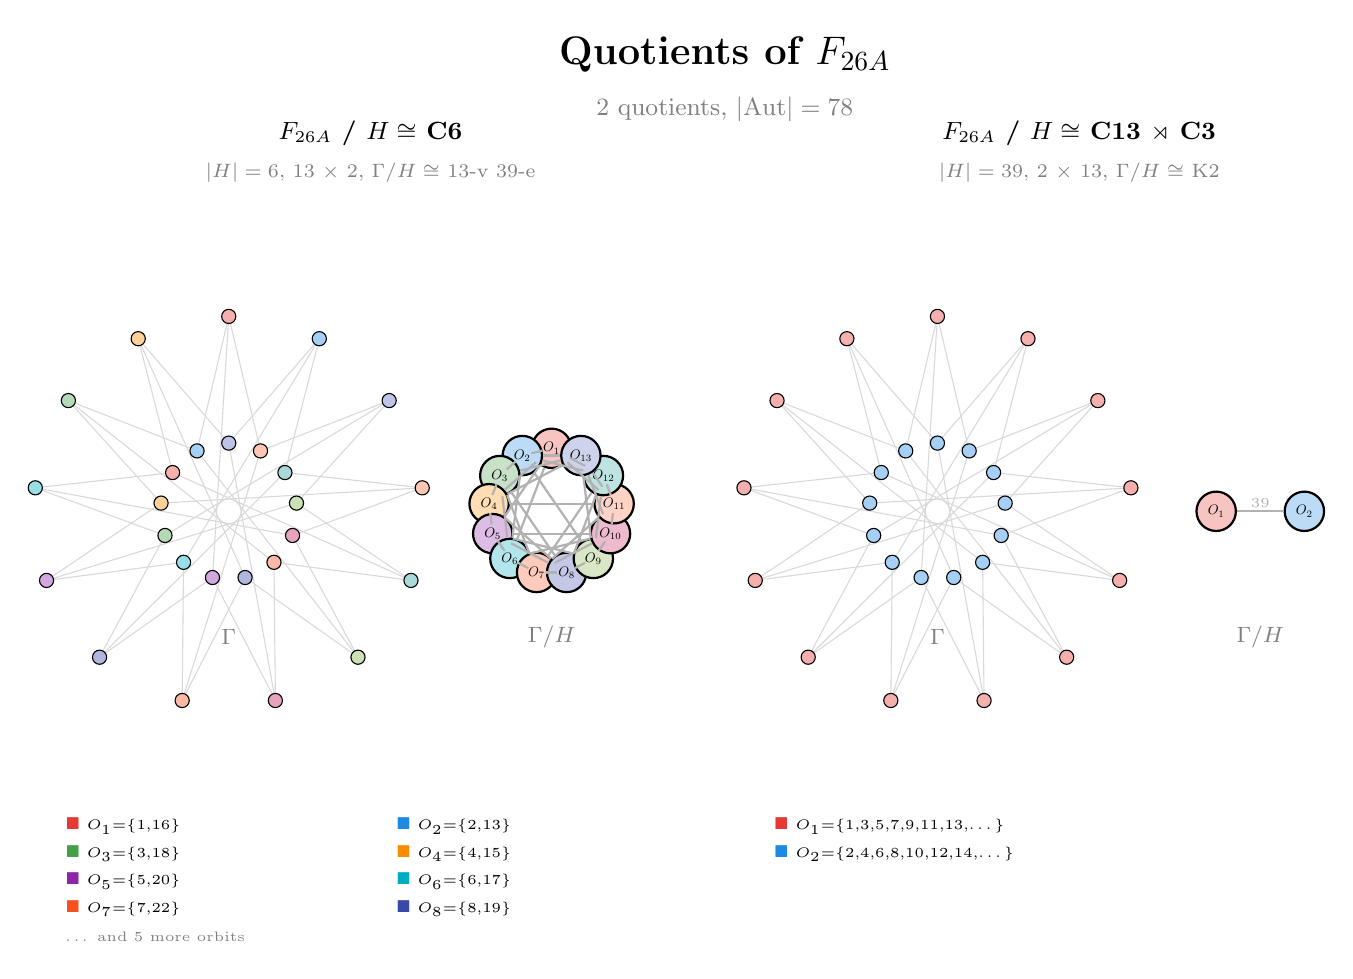
\begin{tikzpicture}[
  ov/.style={circle, draw, semithick, minimum size=3.5mm, inner sep=0pt},
  ovs/.style={circle, draw, thin, minimum size=1.8mm, inner sep=0pt},
  qv/.style={circle, draw, thick, minimum size=5mm, inner sep=0pt},
  cardtitle/.style={font=\small\bfseries},
  cardsub/.style={font=\scriptsize, text=gray},
  glabel/.style={font=\footnotesize, text=gray},
]
\node[font=\Large\bfseries] at (0, 11.5) {Quotients of $F_{26A}$};
\node[font=\small, text=gray] at (0, 10.8) {2 quotients, $|\mathrm{Aut}|=78$};

% Card: $F_{26A}$ / H=C6
\node[cardtitle] at (-4.50,10.50) {$F_{26A}$ / $H \cong$ C6};
\node[cardsub] at (-4.50,10.00) {$|H|=6$, 13 $\times$ 2, $\Gamma/H \cong$ 13-v 39-e};
\draw[gray!30, thin] (-6.300,8.175) -- (-6.703,6.467);
\draw[gray!30, thin] (-6.300,8.175) -- (-6.507,4.859);
\draw[gray!30, thin] (-6.300,8.175) -- (-5.897,6.467);
\draw[gray!30, thin] (-6.703,6.467) -- (-8.337,7.106);
\draw[gray!30, thin] (-6.703,6.467) -- (-4.659,3.847);
\draw[gray!30, thin] (-8.337,7.106) -- (-7.160,5.804);
\draw[gray!30, thin] (-8.337,7.106) -- (-5.726,5.052);
\draw[gray!30, thin] (-7.160,5.804) -- (-8.614,4.822);
\draw[gray!30, thin] (-7.160,5.804) -- (-3.843,5.998);
\draw[gray!30, thin] (-8.614,4.822) -- (-6.874,5.052);
\draw[gray!30, thin] (-8.614,4.822) -- (-5.440,5.804);
\draw[gray!30, thin] (-6.874,5.052) -- (-6.892,3.297);
\draw[gray!30, thin] (-6.874,5.052) -- (-5.150,7.892);
\draw[gray!30, thin] (-6.892,3.297) -- (-6.093,4.859);
\draw[gray!30, thin] (-6.892,3.297) -- (-5.897,6.467);
\draw[gray!30, thin] (-6.093,4.859) -- (-4.659,3.847);
\draw[gray!30, thin] (-6.093,4.859) -- (-7.450,7.892);
\draw[gray!30, thin] (-4.659,3.847) -- (-5.490,5.393);
\draw[gray!30, thin] (-5.490,5.393) -- (-3.843,5.998);
\draw[gray!30, thin] (-5.490,5.393) -- (-8.757,5.998);
\draw[gray!30, thin] (-3.843,5.998) -- (-5.587,6.192);
\draw[gray!30, thin] (-5.587,6.192) -- (-5.150,7.892);
\draw[gray!30, thin] (-5.587,6.192) -- (-7.941,3.847);
\draw[gray!30, thin] (-5.150,7.892) -- (-6.300,6.566);
\draw[gray!30, thin] (-6.300,6.566) -- (-7.450,7.892);
\draw[gray!30, thin] (-6.300,6.566) -- (-5.708,3.297);
\draw[gray!30, thin] (-7.450,7.892) -- (-7.013,6.192);
\draw[gray!30, thin] (-7.013,6.192) -- (-8.757,5.998);
\draw[gray!30, thin] (-7.013,6.192) -- (-3.986,4.822);
\draw[gray!30, thin] (-8.757,5.998) -- (-7.110,5.393);
\draw[gray!30, thin] (-7.110,5.393) -- (-7.941,3.847);
\draw[gray!30, thin] (-7.110,5.393) -- (-4.263,7.106);
\draw[gray!30, thin] (-7.941,3.847) -- (-6.507,4.859);
\draw[gray!30, thin] (-6.507,4.859) -- (-5.708,3.297);
\draw[gray!30, thin] (-5.708,3.297) -- (-5.726,5.052);
\draw[gray!30, thin] (-5.726,5.052) -- (-3.986,4.822);
\draw[gray!30, thin] (-3.986,4.822) -- (-5.440,5.804);
\draw[gray!30, thin] (-5.440,5.804) -- (-4.263,7.106);
\draw[gray!30, thin] (-4.263,7.106) -- (-5.897,6.467);
\node[ovs, fill=c0!40] at (-6.300,8.175) {};
\node[ovs, fill=c1!40] at (-6.703,6.467) {};
\node[ovs, fill=c2!40] at (-8.337,7.106) {};
\node[ovs, fill=c3!40] at (-7.160,5.804) {};
\node[ovs, fill=c4!40] at (-8.614,4.822) {};
\node[ovs, fill=c5!40] at (-6.874,5.052) {};
\node[ovs, fill=c6!40] at (-6.892,3.297) {};
\node[ovs, fill=c7!40] at (-6.093,4.859) {};
\node[ovs, fill=c8!40] at (-4.659,3.847) {};
\node[ovs, fill=c9!40] at (-5.490,5.393) {};
\node[ovs, fill=c10!40] at (-3.843,5.998) {};
\node[ovs, fill=c11!40] at (-5.587,6.192) {};
\node[ovs, fill=c1!40] at (-5.150,7.892) {};
\node[ovs, fill=c12!40] at (-6.300,6.566) {};
\node[ovs, fill=c3!40] at (-7.450,7.892) {};
\node[ovs, fill=c0!40] at (-7.013,6.192) {};
\node[ovs, fill=c5!40] at (-8.757,5.998) {};
\node[ovs, fill=c2!40] at (-7.110,5.393) {};
\node[ovs, fill=c7!40] at (-7.941,3.847) {};
\node[ovs, fill=c4!40] at (-6.507,4.859) {};
\node[ovs, fill=c9!40] at (-5.708,3.297) {};
\node[ovs, fill=c6!40] at (-5.726,5.052) {};
\node[ovs, fill=c11!40] at (-3.986,4.822) {};
\node[ovs, fill=c8!40] at (-5.440,5.804) {};
\node[ovs, fill=c12!40] at (-4.263,7.106) {};
\node[ovs, fill=c10!40] at (-5.897,6.467) {};
\node[glabel] at (-6.30,4.10) {$\Gamma$};
\node[qv, fill=c0!30] (c16o0) at (-2.200,6.500) {\scalebox{0.5}{$O_{1}$}};
\node[qv, fill=c1!30] (c16o1) at (-2.572,6.408) {\scalebox{0.5}{$O_{2}$}};
\node[qv, fill=c2!30] (c16o2) at (-2.858,6.154) {\scalebox{0.5}{$O_{3}$}};
\node[qv, fill=c3!30] (c16o3) at (-2.994,5.796) {\scalebox{0.5}{$O_{4}$}};
\node[qv, fill=c4!30] (c16o4) at (-2.948,5.416) {\scalebox{0.5}{$O_{5}$}};
\node[qv, fill=c5!30] (c16o5) at (-2.730,5.101) {\scalebox{0.5}{$O_{6}$}};
\node[qv, fill=c6!30] (c16o6) at (-2.391,4.923) {\scalebox{0.5}{$O_{7}$}};
\node[qv, fill=c7!30] (c16o7) at (-2.009,4.923) {\scalebox{0.5}{$O_{8}$}};
\node[qv, fill=c8!30] (c16o8) at (-1.670,5.101) {\scalebox{0.5}{$O_{9}$}};
\node[qv, fill=c9!30] (c16o9) at (-1.452,5.416) {\scalebox{0.5}{$O_{10}$}};
\node[qv, fill=c10!30] (c16o10) at (-1.406,5.796) {\scalebox{0.5}{$O_{11}$}};
\node[qv, fill=c11!30] (c16o11) at (-1.542,6.154) {\scalebox{0.5}{$O_{12}$}};
\node[qv, fill=c12!30] (c16o12) at (-1.828,6.408) {\scalebox{0.5}{$O_{13}$}};
\draw[gray!60, thick] (c16o0) -- (c16o1);
\draw[gray!60, thick] (c16o0) -- (c16o3);
\draw[gray!60, thick] (c16o0) -- (c16o4);
\draw[gray!60, thick] (c16o0) -- (c16o5);
\draw[gray!60, thick] (c16o0) -- (c16o10);
\draw[gray!60, thick] (c16o0) -- (c16o11);
\draw[gray!60, thick] (c16o1) -- (c16o2);
\draw[gray!60, thick] (c16o1) -- (c16o5);
\draw[gray!60, thick] (c16o1) -- (c16o8);
\draw[gray!60, thick] (c16o1) -- (c16o11);
\draw[gray!60, thick] (c16o1) -- (c16o12);
\draw[gray!60, thick] (c16o2) -- (c16o3);
\draw[gray!60, thick] (c16o2) -- (c16o5);
\draw[gray!60, thick] (c16o2) -- (c16o6);
\draw[gray!60, thick] (c16o2) -- (c16o7);
\draw[gray!60, thick] (c16o2) -- (c16o12);
\draw[gray!60, thick] (c16o3) -- (c16o4);
\draw[gray!60, thick] (c16o3) -- (c16o7);
\draw[gray!60, thick] (c16o3) -- (c16o10);
\draw[gray!60, thick] (c16o3) -- (c16o12);
\draw[gray!60, thick] (c16o4) -- (c16o5);
\draw[gray!60, thick] (c16o4) -- (c16o7);
\draw[gray!60, thick] (c16o4) -- (c16o8);
\draw[gray!60, thick] (c16o4) -- (c16o9);
\draw[gray!60, thick] (c16o5) -- (c16o6);
\draw[gray!60, thick] (c16o5) -- (c16o9);
\draw[gray!60, thick] (c16o6) -- (c16o7);
\draw[gray!60, thick] (c16o6) -- (c16o9);
\draw[gray!60, thick] (c16o6) -- (c16o10);
\draw[gray!60, thick] (c16o6) -- (c16o11);
\draw[gray!60, thick] (c16o7) -- (c16o8);
\draw[gray!60, thick] (c16o7) -- (c16o11);
\draw[gray!60, thick] (c16o8) -- (c16o9);
\draw[gray!60, thick] (c16o8) -- (c16o11);
\draw[gray!60, thick] (c16o8) -- (c16o12);
\draw[gray!60, thick] (c16o9) -- (c16o10);
\draw[gray!60, thick] (c16o9) -- (c16o12);
\draw[gray!60, thick] (c16o10) -- (c16o11);
\draw[gray!60, thick] (c16o10) -- (c16o12);
\node[glabel] at (-2.20,4.10) {$\Gamma/H$};
\node[anchor=west, font=\tiny] at (-8.50,1.70) {\textcolor{c0}{$\blacksquare$} $O_{1}$=\{1,16\}};
\node[anchor=west, font=\tiny] at (-4.30,1.70) {\textcolor{c1}{$\blacksquare$} $O_{2}$=\{2,13\}};
\node[anchor=west, font=\tiny] at (-8.50,1.35) {\textcolor{c2}{$\blacksquare$} $O_{3}$=\{3,18\}};
\node[anchor=west, font=\tiny] at (-4.30,1.35) {\textcolor{c3}{$\blacksquare$} $O_{4}$=\{4,15\}};
\node[anchor=west, font=\tiny] at (-8.50,1.00) {\textcolor{c4}{$\blacksquare$} $O_{5}$=\{5,20\}};
\node[anchor=west, font=\tiny] at (-4.30,1.00) {\textcolor{c5}{$\blacksquare$} $O_{6}$=\{6,17\}};
\node[anchor=west, font=\tiny] at (-8.50,0.65) {\textcolor{c6}{$\blacksquare$} $O_{7}$=\{7,22\}};
\node[anchor=west, font=\tiny] at (-4.30,0.65) {\textcolor{c7}{$\blacksquare$} $O_{8}$=\{8,19\}};
\node[anchor=west, font=\tiny, text=gray] at (-8.50,0.30) {\ldots\ and 5 more orbits};

% Card: $F_{26A}$ / H=C13 : C3
\node[cardtitle] at (4.50,10.50) {$F_{26A}$ / $H \cong$ C13 $\rtimes$ C3};
\node[cardsub] at (4.50,10.00) {$|H|=39$, 2 $\times$ 13, $\Gamma/H \cong$ K2};
\draw[gray!30, thin] (2.700,8.175) -- (2.297,6.467);
\draw[gray!30, thin] (2.700,8.175) -- (2.493,4.859);
\draw[gray!30, thin] (2.700,8.175) -- (3.103,6.467);
\draw[gray!30, thin] (2.297,6.467) -- (0.663,7.106);
\draw[gray!30, thin] (2.297,6.467) -- (4.341,3.847);
\draw[gray!30, thin] (0.663,7.106) -- (1.840,5.804);
\draw[gray!30, thin] (0.663,7.106) -- (3.274,5.052);
\draw[gray!30, thin] (1.840,5.804) -- (0.386,4.822);
\draw[gray!30, thin] (1.840,5.804) -- (5.157,5.998);
\draw[gray!30, thin] (0.386,4.822) -- (2.126,5.052);
\draw[gray!30, thin] (0.386,4.822) -- (3.560,5.804);
\draw[gray!30, thin] (2.126,5.052) -- (2.108,3.297);
\draw[gray!30, thin] (2.126,5.052) -- (3.850,7.892);
\draw[gray!30, thin] (2.108,3.297) -- (2.907,4.859);
\draw[gray!30, thin] (2.108,3.297) -- (3.103,6.467);
\draw[gray!30, thin] (2.907,4.859) -- (4.341,3.847);
\draw[gray!30, thin] (2.907,4.859) -- (1.550,7.892);
\draw[gray!30, thin] (4.341,3.847) -- (3.510,5.393);
\draw[gray!30, thin] (3.510,5.393) -- (5.157,5.998);
\draw[gray!30, thin] (3.510,5.393) -- (0.243,5.998);
\draw[gray!30, thin] (5.157,5.998) -- (3.413,6.192);
\draw[gray!30, thin] (3.413,6.192) -- (3.850,7.892);
\draw[gray!30, thin] (3.413,6.192) -- (1.059,3.847);
\draw[gray!30, thin] (3.850,7.892) -- (2.700,6.566);
\draw[gray!30, thin] (2.700,6.566) -- (1.550,7.892);
\draw[gray!30, thin] (2.700,6.566) -- (3.292,3.297);
\draw[gray!30, thin] (1.550,7.892) -- (1.987,6.192);
\draw[gray!30, thin] (1.987,6.192) -- (0.243,5.998);
\draw[gray!30, thin] (1.987,6.192) -- (5.014,4.822);
\draw[gray!30, thin] (0.243,5.998) -- (1.890,5.393);
\draw[gray!30, thin] (1.890,5.393) -- (1.059,3.847);
\draw[gray!30, thin] (1.890,5.393) -- (4.737,7.106);
\draw[gray!30, thin] (1.059,3.847) -- (2.493,4.859);
\draw[gray!30, thin] (2.493,4.859) -- (3.292,3.297);
\draw[gray!30, thin] (3.292,3.297) -- (3.274,5.052);
\draw[gray!30, thin] (3.274,5.052) -- (5.014,4.822);
\draw[gray!30, thin] (5.014,4.822) -- (3.560,5.804);
\draw[gray!30, thin] (3.560,5.804) -- (4.737,7.106);
\draw[gray!30, thin] (4.737,7.106) -- (3.103,6.467);
\node[ovs, fill=c0!40] at (2.700,8.175) {};
\node[ovs, fill=c1!40] at (2.297,6.467) {};
\node[ovs, fill=c0!40] at (0.663,7.106) {};
\node[ovs, fill=c1!40] at (1.840,5.804) {};
\node[ovs, fill=c0!40] at (0.386,4.822) {};
\node[ovs, fill=c1!40] at (2.126,5.052) {};
\node[ovs, fill=c0!40] at (2.108,3.297) {};
\node[ovs, fill=c1!40] at (2.907,4.859) {};
\node[ovs, fill=c0!40] at (4.341,3.847) {};
\node[ovs, fill=c1!40] at (3.510,5.393) {};
\node[ovs, fill=c0!40] at (5.157,5.998) {};
\node[ovs, fill=c1!40] at (3.413,6.192) {};
\node[ovs, fill=c0!40] at (3.850,7.892) {};
\node[ovs, fill=c1!40] at (2.700,6.566) {};
\node[ovs, fill=c0!40] at (1.550,7.892) {};
\node[ovs, fill=c1!40] at (1.987,6.192) {};
\node[ovs, fill=c0!40] at (0.243,5.998) {};
\node[ovs, fill=c1!40] at (1.890,5.393) {};
\node[ovs, fill=c0!40] at (1.059,3.847) {};
\node[ovs, fill=c1!40] at (2.493,4.859) {};
\node[ovs, fill=c0!40] at (3.292,3.297) {};
\node[ovs, fill=c1!40] at (3.274,5.052) {};
\node[ovs, fill=c0!40] at (5.014,4.822) {};
\node[ovs, fill=c1!40] at (3.560,5.804) {};
\node[ovs, fill=c0!40] at (4.737,7.106) {};
\node[ovs, fill=c1!40] at (3.103,6.467) {};
\node[glabel] at (2.70,4.10) {$\Gamma$};
\node[qv, fill=c0!30] (c17o0) at (6.240,5.700) {\scalebox{0.5}{$O_{1}$}};
\node[qv, fill=c1!30] (c17o1) at (7.360,5.700) {\scalebox{0.5}{$O_{2}$}};
\draw[gray!60, thick] (c17o0) -- node[font=\tiny, auto, inner sep=1pt] {39} (c17o1);
\node[glabel] at (6.80,4.10) {$\Gamma/H$};
\node[anchor=west, font=\tiny] at (0.50,1.70) {\textcolor{c0}{$\blacksquare$} $O_{1}$=\{1,3,5,7,9,11,13,\ldots\}};
\node[anchor=west, font=\tiny] at (0.50,1.35) {\textcolor{c1}{$\blacksquare$} $O_{2}$=\{2,4,6,8,10,12,14,\ldots\}};
\end{tikzpicture}
\end{center}
\clearpage

\begin{center}
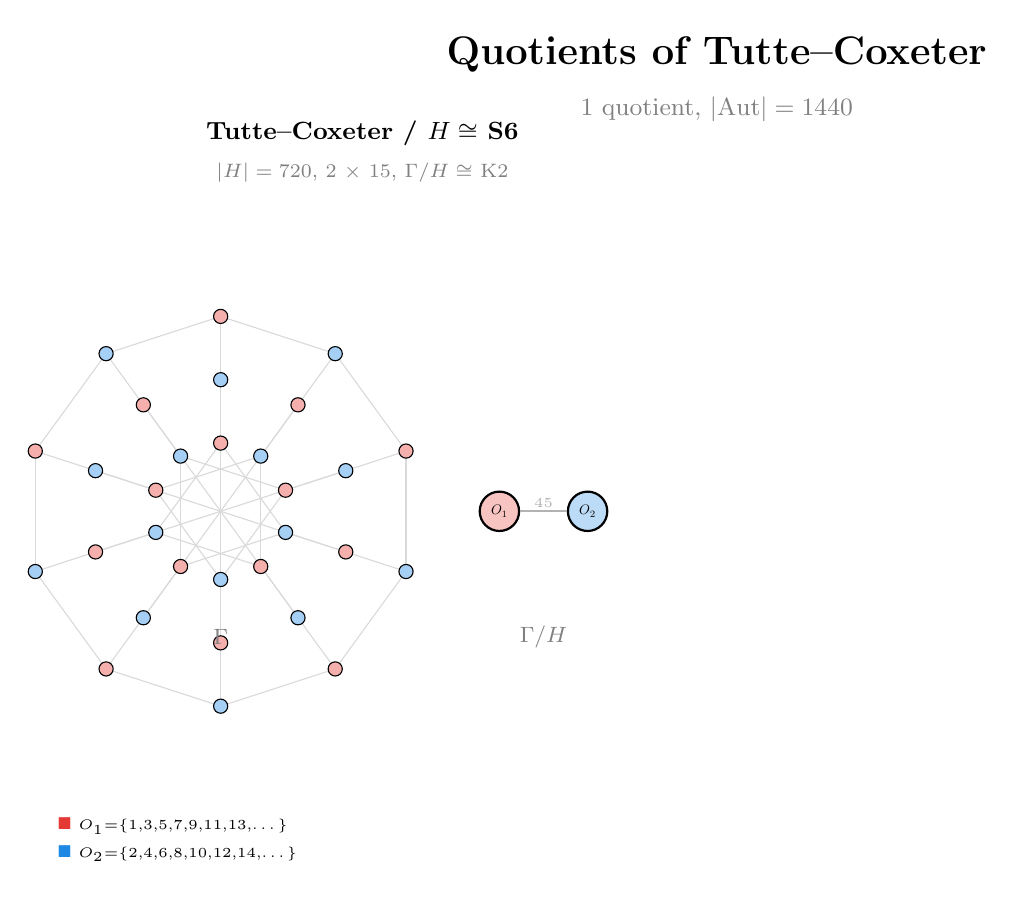
\begin{tikzpicture}[
  ov/.style={circle, draw, semithick, minimum size=3.5mm, inner sep=0pt},
  ovs/.style={circle, draw, thin, minimum size=1.8mm, inner sep=0pt},
  qv/.style={circle, draw, thick, minimum size=5mm, inner sep=0pt},
  cardtitle/.style={font=\small\bfseries},
  cardsub/.style={font=\scriptsize, text=gray},
  glabel/.style={font=\footnotesize, text=gray},
]
\node[font=\Large\bfseries] at (0, 11.5) {Quotients of Tutte--Coxeter};
\node[font=\small, text=gray] at (0, 10.8) {1 quotient, $|\mathrm{Aut}|=1440$};

% Card: Tutte--Coxeter / H=S6
\node[cardtitle] at (-4.50,10.50) {Tutte--Coxeter / $H \cong$ S6};
\node[cardsub] at (-4.50,10.00) {$|H|=720$, 2 $\times$ 15, $\Gamma/H \cong$ K2};
\draw[gray!30, thin] (-6.300,8.175) -- (-7.755,7.702);
\draw[gray!30, thin] (-6.300,8.175) -- (-6.300,7.371);
\draw[gray!30, thin] (-6.300,8.175) -- (-4.845,7.702);
\draw[gray!30, thin] (-7.755,7.702) -- (-8.654,6.465);
\draw[gray!30, thin] (-7.755,7.702) -- (-7.282,7.052);
\draw[gray!30, thin] (-8.654,6.465) -- (-8.654,4.935);
\draw[gray!30, thin] (-8.654,6.465) -- (-7.889,6.216);
\draw[gray!30, thin] (-8.654,4.935) -- (-7.755,3.698);
\draw[gray!30, thin] (-8.654,4.935) -- (-7.889,5.184);
\draw[gray!30, thin] (-7.755,3.698) -- (-6.300,3.225);
\draw[gray!30, thin] (-7.755,3.698) -- (-7.282,4.348);
\draw[gray!30, thin] (-6.300,3.225) -- (-4.845,3.698);
\draw[gray!30, thin] (-6.300,3.225) -- (-6.300,4.029);
\draw[gray!30, thin] (-4.845,3.698) -- (-3.946,4.935);
\draw[gray!30, thin] (-4.845,3.698) -- (-5.318,4.348);
\draw[gray!30, thin] (-3.946,4.935) -- (-4.711,5.184);
\draw[gray!30, thin] (-3.946,4.935) -- (-3.946,6.465);
\draw[gray!30, thin] (-4.711,5.184) -- (-7.889,6.216);
\draw[gray!30, thin] (-4.711,5.184) -- (-5.476,5.432);
\draw[gray!30, thin] (-7.889,6.216) -- (-7.124,5.968);
\draw[gray!30, thin] (-7.124,5.968) -- (-5.791,6.401);
\draw[gray!30, thin] (-7.124,5.968) -- (-6.300,4.834);
\draw[gray!30, thin] (-5.791,6.401) -- (-5.318,7.052);
\draw[gray!30, thin] (-5.791,6.401) -- (-5.791,4.999);
\draw[gray!30, thin] (-5.318,7.052) -- (-7.282,4.348);
\draw[gray!30, thin] (-5.318,7.052) -- (-4.845,7.702);
\draw[gray!30, thin] (-7.282,4.348) -- (-6.809,4.999);
\draw[gray!30, thin] (-6.809,4.999) -- (-5.476,5.432);
\draw[gray!30, thin] (-6.809,4.999) -- (-6.809,6.401);
\draw[gray!30, thin] (-5.476,5.432) -- (-6.300,6.566);
\draw[gray!30, thin] (-6.300,6.566) -- (-6.300,7.371);
\draw[gray!30, thin] (-6.300,6.566) -- (-7.124,5.432);
\draw[gray!30, thin] (-6.300,7.371) -- (-6.300,4.029);
\draw[gray!30, thin] (-6.300,4.029) -- (-6.300,4.834);
\draw[gray!30, thin] (-6.300,4.834) -- (-5.476,5.968);
\draw[gray!30, thin] (-5.476,5.968) -- (-6.809,6.401);
\draw[gray!30, thin] (-5.476,5.968) -- (-4.711,6.216);
\draw[gray!30, thin] (-6.809,6.401) -- (-7.282,7.052);
\draw[gray!30, thin] (-7.282,7.052) -- (-5.318,4.348);
\draw[gray!30, thin] (-5.318,4.348) -- (-5.791,4.999);
\draw[gray!30, thin] (-5.791,4.999) -- (-7.124,5.432);
\draw[gray!30, thin] (-7.124,5.432) -- (-7.889,5.184);
\draw[gray!30, thin] (-7.889,5.184) -- (-4.711,6.216);
\draw[gray!30, thin] (-4.711,6.216) -- (-3.946,6.465);
\draw[gray!30, thin] (-3.946,6.465) -- (-4.845,7.702);
\node[ovs, fill=c0!40] at (-6.300,8.175) {};
\node[ovs, fill=c1!40] at (-7.755,7.702) {};
\node[ovs, fill=c0!40] at (-8.654,6.465) {};
\node[ovs, fill=c1!40] at (-8.654,4.935) {};
\node[ovs, fill=c0!40] at (-7.755,3.698) {};
\node[ovs, fill=c1!40] at (-6.300,3.225) {};
\node[ovs, fill=c0!40] at (-4.845,3.698) {};
\node[ovs, fill=c1!40] at (-3.946,4.935) {};
\node[ovs, fill=c0!40] at (-4.711,5.184) {};
\node[ovs, fill=c1!40] at (-7.889,6.216) {};
\node[ovs, fill=c0!40] at (-7.124,5.968) {};
\node[ovs, fill=c1!40] at (-5.791,6.401) {};
\node[ovs, fill=c0!40] at (-5.318,7.052) {};
\node[ovs, fill=c1!40] at (-7.282,4.348) {};
\node[ovs, fill=c0!40] at (-6.809,4.999) {};
\node[ovs, fill=c1!40] at (-5.476,5.432) {};
\node[ovs, fill=c0!40] at (-6.300,6.566) {};
\node[ovs, fill=c1!40] at (-6.300,7.371) {};
\node[ovs, fill=c0!40] at (-6.300,4.029) {};
\node[ovs, fill=c1!40] at (-6.300,4.834) {};
\node[ovs, fill=c0!40] at (-5.476,5.968) {};
\node[ovs, fill=c1!40] at (-6.809,6.401) {};
\node[ovs, fill=c0!40] at (-7.282,7.052) {};
\node[ovs, fill=c1!40] at (-5.318,4.348) {};
\node[ovs, fill=c0!40] at (-5.791,4.999) {};
\node[ovs, fill=c1!40] at (-7.124,5.432) {};
\node[ovs, fill=c0!40] at (-7.889,5.184) {};
\node[ovs, fill=c1!40] at (-4.711,6.216) {};
\node[ovs, fill=c0!40] at (-3.946,6.465) {};
\node[ovs, fill=c1!40] at (-4.845,7.702) {};
\node[glabel] at (-6.30,4.10) {$\Gamma$};
\node[qv, fill=c0!30] (c18o0) at (-2.760,5.700) {\scalebox{0.5}{$O_{1}$}};
\node[qv, fill=c1!30] (c18o1) at (-1.640,5.700) {\scalebox{0.5}{$O_{2}$}};
\draw[gray!60, thick] (c18o0) -- node[font=\tiny, auto, inner sep=1pt] {45} (c18o1);
\node[glabel] at (-2.20,4.10) {$\Gamma/H$};
\node[anchor=west, font=\tiny] at (-8.50,1.70) {\textcolor{c0}{$\blacksquare$} $O_{1}$=\{1,3,5,7,9,11,13,\ldots\}};
\node[anchor=west, font=\tiny] at (-8.50,1.35) {\textcolor{c1}{$\blacksquare$} $O_{2}$=\{2,4,6,8,10,12,14,\ldots\}};
\end{tikzpicture}
\end{center}
\clearpage
\end{document}